\documentclass{article}

% if you need to pass options to natbib, use, e.g.:
%     \PassOptionsToPackage{numbers, compress}{natbib}
% before loading neurips_2026

% The authors should use one of these tracks.
% Before accepting by the NeurIPS conference, select one of the options below.
% 0. "default" for submission
%\usepackage[preprint]{neurips_2026}
% the "default" option is equal to the "main" option, which is used for the Main Track with double-blind reviewing.
% 1. "main" option is used for the Main Track
%  \usepackage[main]{neurips_2026}
% 2. "position" option is used for the Position Paper Track
%  \usepackage[position]{neurips_2026}
% 3. "eandd" option is used for the Evaluations & Datasets Track
 % \usepackage[eandd]{neurips_2026}
% 4. "creativeai" option is used for the Creative AI Track
%  \usepackage[creativeai]{neurips_2026}
% 5. "sglblindworkshop" option is used for the Workshop with single-blind reviewing
 % \usepackage[sglblindworkshop]{neurips_2026}
% 6. "dblblindworkshop" option is used for the Workshop with double-blind reviewing
%  \usepackage[dblblindworkshop]{neurips_2026}

% After being accepted, the authors should add "final" behind the track to compile a camera-ready version.
% 1. Main Track
 % \usepackage[main, final]{neurips_2026}
% 2. Position Paper Track
%  \usepackage[position, final]{neurips_2026}
% 3. Evaluations & Datasets Track
 % \usepackage[eandd, final]{neurips_2026}
% 4. Creative AI Track
%  \usepackage[creativeai, final]{neurips_2026}
% 5. Workshop with single-blind reviewing
%  \usepackage[sglblindworkshop, final]{neurips_2026}
% 6. Workshop with double-blind reviewing
%  \usepackage[dblblindworkshop, final]{neurips_2026}
% Note. For the workshop paper template, both \title{} and \workshoptitle{} are required, with the former indicating the paper title shown in the title and the latter indicating the workshop title displayed in the footnote.
% For workshops (5., 6.), the authors should add the name of the workshop, "\workshoptitle" command is used to set the workshop title.
% \workshoptitle{WORKSHOP TITLE}

% "preprint" option is used for arXiv or other preprint submissions
 % \usepackage[preprint]{neurips_2026}

% to avoid loading the natbib package, add option nonatbib:
%    \usepackage[nonatbib]{neurips_2026}

\usepackage[utf8]{inputenc} % allow utf-8 input
\usepackage[T1]{fontenc}    % use 8-bit T1 fonts
\usepackage[numbers,sort&compress]{natbib} % numbered literature citations
\usepackage{hyperref}       % hyperlinks
\usepackage{url}            % simple URL typesetting
\usepackage{booktabs}       % professional-quality tables
\usepackage{amsfonts}       % blackboard math symbols
\usepackage{amsmath}        % align, cases, \text
\usepackage{nicefrac}       % compact symbols for 1/2, etc.
\usepackage{microtype}      % microtypography
\usepackage{xcolor}         % colors
\usepackage{graphicx}       % figures
\usepackage[font=small,labelfont=bf]{caption}

\providecommand{\doi}[1]{\href{https://doi.org/#1}{doi:\nolinkurl{#1}}}

\graphicspath{{figure/}{../data/}{data/}}

% Note. For the workshop paper template, both \title{} and \workshoptitle{} are required, with the former indicating the paper title shown in the title and the latter indicating the workshop title displayed in the footnote. 
\title{Statistical Mechanics of Turing Machines}


% The \author macro works with any number of authors. There are two commands
% used to separate the names and addresses of multiple authors: \And and \AND.
%
% Using \And between authors leaves it to LaTeX to determine where to break the
% lines. Using \AND forces a line break at that point. So, if LaTeX puts 3 of 4
% authors names on the first line, and the last on the second line, try using
% \AND instead of \And before the third author name.


\author{%
  Tankut ~Can\\
  Department of Physics\\
  Emory University\\
  Atlanta, GA 30022 \\
  \texttt{tcan@emory.edu} \\
  % examples of more authors
  % \And
  % Coauthor \\
  % Affiliation \\
  % Address \\
  % \texttt{email} \\
  % \AND
  % Coauthor \\
  % Affiliation \\
  % Address \\
  % \texttt{email} \\
  % \And
  % Coauthor \\
  % Affiliation \\
  % Address \\
  % \texttt{email} \\
  % \And
  % Coauthor \\
  % Affiliation \\
  % Address \\
  % \texttt{email} \\
}


\begin{document}


\maketitle
\tableofcontents

\section{Turing Machines}
\label{sec:turing-machines}

I will define the basic objects I'm working with. I will treat a single Turing Machine as a dynamical system. In order to describe it, I need three variables: 1) The tape value at time step $t$ and position $x$ on the tape $V_{t}(x) \in [s] = \{ 0, 1, ..., s-1\}$. This a Turing machine that can write any symbol from a set of $s$ symbols; 2) The position of the Turing Machine on this tape $x_{t} \in \mathbb{Z}$. For the moment, I'm assuming an infinite tape, but it might be necessary to consider periodic boundary conditions, in which case $x_{t} \in \mathbb{Z}_{L}$; 3) The state of the TM $q_{t} \in [ n] : = \{ 1, 2, ..., n\}$ for a $n-$state TM. To denote a Turing machine with $n$ states over $s$ symbols we write ${\rm TM}_{n}(s)$. I will focus mostly on ${\rm TM}_{n}(2)$, for which the tape consists of $\{0,1\}$, but the TM can have arbitrarily many states. 


The equations of motion of a single Turing machine are


\begin{align}
x_{t+1} &= x_{t} +M_{q_{t}}\left( V_{t}(x_{t})\right)\\
V_{t+1}(x_{t}) & = W_{q_{t}}\left( V_{t}(x_{t})\right)\\
q_{t+1} & = S_{q_{t}}\left( V_{t}(x_{t})\right)
\end{align}

This is the most general formulation, and illustrates the fact that to define a TM we require three equal-sized matrices $M, W, S$. For each index $q_{t}$, the rows of these matrices define a function from the value of the tape that is read $V_{t}(x_{t})$, to the corresponding response. $M$ gives the next move, and so $M_{q}(b) \in \{-1, +1\}$. $W$ gives the symbol that is written, so $W_{q}(b) \in [ s]$. Finally, $S$ tells the TM which state to transition to after being in state $q_{t}$ and reading tape value $V_{t}(x_{t})$. For this reason, $S_{q}(b) \in [n]$, 




\section{Langton's Ant}
\label{sec:langton-ant}

The first simple example we start with is Langton's ant, also called a turmite (presumably a portmanteau of turing and mite). Typically these are studied on a 2D grid, but I consider them on a one-dimensional tape. This model belongs to the class of ${\rm TM}_{1}(2)$, since there is only a single state and the behavior ultimately depends only on the current state of the tape. The rules are:


$$\begin{array}{ccc}
{\rm Read} & {\rm Write} & {\rm Move} \\
0 & 1 & Left\\
1 & 0 & Right
\end{array}$$

For a single turmite, using the notation above, the update rules are

\begin{align}
x_{t+1}^{\mu} &= x_{t}^{\mu} + 2 V_{t}(x_{t}^{\mu}) - 1\\
V_{t+1}(x_{t}^{\mu}) & = 1 - V_{t}(x_{t}^{\mu})
\end{align}

There is a nicer representation in terms of the function $V_{t}(x)$, and the number of termites at $x$ at time $t$:

\begin{align}
n_{t}(x) = \sum_{\mu = 1}^{N} \delta_{x \, x_{t}^{\mu}}
\end{align}

Without any explicit exclusion rule, there can be any number of turmites at a site, and their actions will all be in perfect agreement, so there is no risk of contradiction or interference. Note that with turing machine, one needs to add a rule about how conflicts are resolved, since adjacent TMs might be in different states, and consequently will want to take contradictory write actions on the same location. 

Back to the turmite, we can find update rules for the tape value function and the density of turmites:

\begin{align}
V_{t+1}(x) &= V_{t}(x) + \Theta(n_{t}(x)) \left(1 - 2 V_{t}(x)\right)\\
n_{t+1}(x)  & =  \left(1 - V_{t}(x+1)\right) n_{t}(x + 1) + V_{t}(x - 1) n_{t}(x - 1)
\end{align}

where $\Theta(n_{t}(x)) = 1$ for $n_{t}(x) > 0$ and $0$ otherwise. The total number of turmites never changes, and so $N = \sum_{x} n_{t}(x)$ is conserved. This implies at least a continuity equation. Let's define the chiral current flux. In the right direction, let $J_{R}(x-1, x)$ denote the total flux from $x-1$ to $x$. This just

\begin{align}
J_{R}(x-1, x) = V_{t}(x-1) n_{t}(x-1) - (1 - V_{t}(x)) n_{t}(x)
\end{align}

Similarity, the leftward flux from $x+1$ to $x$ is

\begin{align}
J_{L}(x+1, x) = (1 - V_{t}(x+1)) n_{t}(x+1) - V_{t}(x) n_{t}(x) = - J_{R}(x, x+1)
\end{align}

Using these fluxes, I get

\begin{align}
n_{t+1}(x) - n_{t}(x)  & = J_{R}(x-1, x) + J_{L}(x+1, x) = J_{R}(x-1, x) - J_{R}(x, x+1)
\end{align}
 which is the discrete version of the continuity equation. There is a different presentation of this in the appendix. 
 
 
\subsection{Turmitic Solitons}

The simulations suggest looking for solitonic solutions which are ballistic. Let us assume that $n_{t}(x) = N \delta_{x 0}$ for a doubly infinite tape, and $V_{t}(x) = 1$ . Then

\begin{align}
V_{t+1}(0) = 0, \quad n_{t+1}(1) = N, \quad n_{t+1}(0) = 0\\
V_{t+2}(1) = 0, \quad n_{t+2}(2) = N, \quad n_{t+2}(1) = 0
\end{align}
 
 In general, let's just assume initial $t = 0$. Then
 
 \begin{align}
 V_{t}(x) = \sum_{x' < t} \delta_{x, x'}, \quad n_{t}(x) = N\delta_{x, t}
 \end{align}
 Which is clearly a soliton moving at velocity $v = 1$. Now let's say that $V_{0}(x) = 0$ for $x > L$. Then this soliton will move until it hits $x = L$, then it will be reflected and start moving at $v = 1$ in the opposite direction. 
 
 Another thing to notice: If all turmites occupy the same point, there is no mechanism for them to disperse. Therefore, unless the individual turmites never collide, the most likely asymptotic configuration is for all of the turmites to coalesce into one multi-cellular monster, moving as a soliton throughout the tape. 


\section{Simplest Turing Machines}

Now let's try to extend the analysis of Langton's ant to simple 2 state turing machines. 


\newpage


\appendix
\section*{AI scratchpad}



\section{Prior Works}
\label{sec:prior-works}

The systems considered here consist of mobile finite-state machines that
read and modify a shared tape.  Their collective behavior connects several
existing research programs: cellular automata, interacting turmites,
algorithmic chemistry, deterministic walks in a writable environment, and
nonequilibrium statistical mechanics.  The distinction between these
connections matters.  Some references study nearly the same microscopic
architecture; others supply observables or solution methods whose
assumptions must be checked for the present dynamics.

\subsection{Cellular automata, mobile automata, and rule-space surveys}

Wolfram's statistical-mechanical study of cellular
automata~\citep{wolfram1983statistical} is a methodological precedent for
sampling simple deterministic rules, evolving random initial conditions,
and comparing the resulting organization.  It demonstrates that local
binary rules can generate structured statistical behavior without an
equilibrium energy function.  In a cellular automaton, the sites update
through a prescribed spatial rule; in the present simulations, the moving
heads determine where updates occur.  Their positions therefore form an
additional dynamical field.

\emph{A New Kind of Science}~\citep{wolfram2002nks} extends systematic
experimentation to Turing machines and mobile automata, including generalized
mobile automata with multiple active cells.  These examples motivate the
spacetime zoos and comparisons between blank and random tapes.  The
associated 2003 collection of open problems~\citep{wolfram2003open} calls
for systematic studies of simple Turing machines, nonblank initial
conditions, and the relation between active-cell density and behavioral
complexity.  Those historical questions closely match the present program,
but their appearance in that collection does not establish their current
research status.  Wolfram's later multiway Turing
machines~\citep{wolfram2021multiway} concern branching computational
histories under nondeterministic rules.  Multiple branches are distinct
from a population of heads simultaneously modifying a single tape.

\subsection{Interacting turmites and shared-tape agents}

Belgacem and Fat\`es~\citep{belgacem2012turmites} provide a direct spatial
precedent by studying multiple Langton turmites on a shared binary lattice.
They compare synchronous updates, a fixed sequential order, and random
sequential orders, together with different policies for spatial conflicts.
Their experiments show that collective patterns depend on the scheduling
and interaction conventions, even when the individual agent rule stays
fixed.  This supports treating update order and collision resolution as
model parameters in our simulations.  Their model is two-dimensional and
includes agent orientation and movement-conflict policies, so its
collective structures do not directly determine the behavior of the
one-dimensional rules studied below.

Polhill and collaborators~\citep{polhill2021prediction} explicitly consider
a population of Turing machines reading and writing the same tape.  Their
thought experiment studies prediction when transition tables, initial head
states and positions, and execution schedules are hidden.  It establishes
a close architectural precedent, while addressing inference and
computability rather than deriving stationary measures or transport laws.
In particular, its discussion of noncomputable schedules should be
distinguished from the reproducible, seeded random schedules used in
numerical experiments here.

\subsection{Algorithmic chemistry and Fontana's Turing gas}

Fontana's algorithmic chemistry~\citep{fontana1991chemistry} treats an
ensemble of symbolic functions as interacting objects.  In this
``Turing gas,'' expressions derived from the lambda calculus act on one
another to generate new expressions, and the population develops
cooperative organizations.  This supplies an early precedent for studying
collective behavior in a population of programs.

Fontana and Buss~\citep{fontana1994tape} subsequently analyze the emergence
of reproducing and self-maintaining organizations in this abstract
chemistry.  Their work suggests examining which interaction patterns
persist across different initial populations.  The correspondence to our
model is conceptual: their reacting objects are themselves programs, and
reactions change the program population.  Here the sampled transition
tables remain fixed and the shared spatial tape carries the evolving
record of interactions.  Thus algorithmic chemistry motivates questions
about collective organization, but its reaction rules cannot be imported
as the dynamics of the present gas.

\subsection{Eulerian walkers and rotor-router theory}

The symbol-flipping one-state machine has a particularly close connection
to rotor walks: successive occupied visits alternate the departure
direction at a site.  Priezzhev and
collaborators~\citep{priezzhev1996eulerian} study walkers that modify local
arrows and, on open graphs, are replaced after absorption.  Their particle
addition operators connect the stationary problem to the Abelian sandpile
model.  Holroyd and collaborators~\citep{holroyd2008rotor} give a systematic
treatment of rotor routing, its Abelian properties, and the relation
between recurrent rotor configurations and rooted spanning trees.

These results apply directly to the isolated-particle excursions used in
the dilute boundary-driven calculation in
Appendix~\ref{sec:boundary-driven}, after matching the convention for
whether a rotor records the last or next departure.  In particular, the
recurrent empty tapes $1^k0^{L-k}$ are the one-dimensional version of
acyclic rotor configurations with absorbing boundaries.  The dilute
calculation should therefore be understood in the context of established
rotor-router theory, rather than as an unrelated mechanism.

Klasing and collaborators~\citep{klasing2017ring} analyze several agents
sharing a rotor environment on a ring, obtaining rigorous cover-time and
long-time return-time results.  A decisive microscopic difference is that
their rotor advances once per departing agent: two agents at one site can
leave in opposite directions.  In our synchronous symbol-flipping model,
the tape flips once per \emph{occupied site}, and all particles in a stack
depart together.  Stacks that meet at one site merge permanently.  The
published multi-agent bounds and Abelian arguments therefore do not
automatically extend to this coalescing dynamics.  They identify useful
tools and solvable sectors, while leaving a distinct problem at finite
stack density.

\subsection{Quantifying tape structure and relaxation}

Computational mechanics provides observables that distinguish visible
organization from simple changes in symbol frequency.  Shalizi and
collaborators~\citep{shalizi2006filters} develop local sensitivity and
statistical-complexity filters for detecting coherent structures in
spatiotemporal systems.  Applied to cellular automata, these reveal domains
and localized structures without assuming their shapes in advance.  For
the present spacetime plots, such filters suggest a way to quantify
traveling structures and collision regions, supplementing head trajectories
and tape density.

Feldman, McTague, and Crutchfield~\citep{feldman2008complexity} compare
processes using complexity--entropy diagrams, combining randomness with
stored structure.  This is relevant because a tape with equal numbers of
zeros and ones can still be periodic or strongly correlated.  Useful
measurements here would include block entropies, entropy rates, excess
entropy, spatial correlations, and correlations between head states and
local symbols.  Estimating them requires specifying the ensemble and
checking stationarity; pooling different machine rules or different ages
of a relaxing system can otherwise obscure the distinction between
within-run fluctuations and variation across runs.  Convergence of these
observables would provide evidence of statistical relaxation, but would not by
itself identify a Gibbs ensemble or a temperature.

\subsection{Boundary-driven states and thermodynamic costs}

The review by Bu\v{c}a, Klobas, and
Prosen~\citep{buca2021rule54} describes exact nonequilibrium stationary
states of the reversible Rule-54 cellular automaton with stochastic
boundaries, including patch and matrix-product representations, relaxation
modes, and current fluctuations.  It supplies a concrete strategy for the
boundary-driven attempt below: specify the reservoirs, construct the
Markov operator, solve small systems, and search for a representation
whose local algebra verifies stationarity.  Its exact formulas depend on
that model's microscopic structure.  Our synchronous coalescence rule
does not inherit those formulas merely because it also admits a
cellular-automaton description.  The transferable object is the
stationary-state problem and the methods used to attack it.

Strasberg and collaborators~\citep{strasberg2015thermodynamics} address a
different thermodynamic question by constructing stochastic physical
implementations of Turing machines with consistent entropy production.
Their results concern the cost of performing computation.  A statistical
ensemble of abstract shared-tape machines does not yet specify the energy
levels, physical transition rates, or reservoirs needed to assign heat
and work.  For this reason, tape Shannon entropy and state-distribution
entropy should initially be treated as information-theoretic observables,
not identified with physical entropy production.

\subsection{Scope of the present problem}

Together, these references establish precedents for computational
populations, agents coupled through writable media, and statistical
descriptions of deterministic local dynamics.  Within the works reviewed
here, we have not identified a general stationary or hydrodynamic theory
covering arbitrary randomly sampled transition tables under the present
shared-tape collision rules; this is a statement about the scope of this
review, not a claim of priority.

A useful formulation separates randomness in the initial tape and head
states from randomness in the transition tables.  Sampling a table once
and retaining it defines quenched algorithmic disorder; resampling it
during evolution would define a different process.  The closed-system
limit should specify particle number $N$, tape length $L$, and density
$N/L$, while an open-system limit must also fix how reservoir rates scale
with $L$.  The one-state symbol-flipping model below isolates a tractable
part of this broader program: it connects directly to rotor walks in the
single-stack sector and introduces irreversible coalescence when several
stacks interact synchronously.




\section{Notes on Langton's Ant}

The rule considered above is
\begin{equation}
0 \longrightarrow (1,L),
\qquad
1 \longrightarrow (0,R).
\end{equation}
It is useful to distinguish the number of turmites at a site from the Boolean
event that the site is occupied.  Define
\begin{equation}
I_t(x) = \mathbf{1}_{\{n_t(x)>0\}}.
\end{equation}
Thus, throughout this section, $\Theta(n)$ is understood to equal zero at
$n=0$ and one for $n>0$.

Under synchronous updating, all turmites first read the tape at time $t$,
then propose their writes and moves.  Since all turmites at a given site read
the same symbol, their write proposals agree.  The exact tape update is
therefore
\begin{align}
V_{t+1}(x)
&= V_t(x) + I_t(x)\left[1-2V_t(x)\right] \\
&= V_t(x) \mathbin{\oplus} I_t(x),
\end{align}
where $\oplus$ denotes addition modulo two.

A turmite at $x+1$ enters $x$ if it reads zero and moves left, whereas a
turmite at $x-1$ enters $x$ if it reads one and moves right.  Consequently,
the exact number update is
\begin{equation}
\boxed{
n_{t+1}(x)
= \left[1-V_t(x+1)\right]n_t(x+1)
+ V_t(x-1)n_t(x-1).
}
\label{eq:exact-number-update}
\end{equation}
This agrees with the number update in the main text.  If the equation is
instead written for the increment $n_{t+1}(x)-n_t(x)$, its right-hand side
must include the additional loss term $-n_t(x)$.

To display number conservation, define the rightward current across the bond
$x+\tfrac12$ by
\begin{equation}
J_t\left(x+\tfrac12\right)
= V_t(x)n_t(x)
- \left[1-V_t(x+1)\right]n_t(x+1).
\end{equation}
The number equation then takes the continuity form
\begin{equation}
n_{t+1}(x)-n_t(x)
= J_t\left(x-\tfrac12\right)-J_t\left(x+\tfrac12\right).
\end{equation}
On an infinite tape with suitable decay, or on a periodic tape with all site
indices understood modulo $L$, this implies
\begin{equation}
\sum_x n_{t+1}(x)=\sum_x n_t(x)=N.
\end{equation}

\subsection{Rotor representation}

Define a binary rotor field
\begin{equation}
\sigma_t(x)=2V_t(x)-1 \in \{-1,+1\},
\end{equation}
where $-1$ sends a stack left and $+1$ sends it right.  The coupled equations
become
\begin{align}
\sigma_{t+1}(x)
&= (-1)^{I_t(x)}\sigma_t(x), \\
n_{t+1}(x)
&= \frac{1-\sigma_t(x+1)}{2}n_t(x+1)
+ \frac{1+\sigma_t(x-1)}{2}n_t(x-1).
\end{align}
The first equation says that an occupied site reverses its rotor exactly once,
independently of the number of turmites in the stack.

The tape and the support of the turmite distribution form a closed Boolean
system.  In particular,
\begin{equation}
\boxed{
I_{t+1}(x)
= \left[I_t(x-1)\land V_t(x-1)\right]
\lor
\left[I_t(x+1)\land \neg V_t(x+1)\right].
}
\end{equation}
Together with $V_{t+1}=V_t\oplus I_t$, this is a deterministic, nearest-neighbor
four-state cellular automaton for $(V_t,I_t)$.  The integer masses $n_t(x)$ can
be transported after the Boolean dynamics have been solved.

Every occupied site sends its entire stack to one neighboring site.  Two
stacks that arrive at the same site merge and can never split again.  Hence
the number of occupied sites
\begin{equation}
K_t=\sum_x I_t(x)
\end{equation}
is nonincreasing:
\begin{equation}
K_{t+1}\leq K_t.
\end{equation}
This monotonic coalescence property is a useful simplification even though the
conserved mass $N$ need not decrease.

\subsection{Odometer representation and a route to a solution}

Introduce the site odometer
\begin{equation}
u_t(x)=\sum_{\tau=0}^{t-1} I_\tau(x),
\end{equation}
which counts the number of time steps at which site $x$ has been occupied.
The tape can then be eliminated in favor of its initial condition:
\begin{equation}
\sigma_t(x)=\sigma_0(x)(-1)^{u_t(x)}.
\end{equation}
For a single stack at position $X_t$, this gives the closed rotor-walk form
\begin{equation}
X_{t+1}
= X_t + \sigma_0(X_t)(-1)^{u_t(X_t)}.
\end{equation}

A possible route toward solving the many-turmite system is the following.
\begin{enumerate}
    \item Solve the single-stack rotor walk in terms of its odometer, visited
    interval, and return times.

    \item Classify two-stack scattering and determine the conditions for
    coalescence.  On an even ring, each step changes position parity, so two
    stacks can occupy the same site at the same time only if their initial
    positions have the same parity.

    \item Analyze the four-state cellular automaton $(V,I)$ on small periodic
    rings by constructing its complete transition graph.  This gives exact
    attractors, periods, traveling waves, and basin sizes without retaining
    the stack masses.

    \item Use the fact that a deterministic system on a finite ring must
    eventually become periodic.  A traveling orbit that advances by $d$
    sites in $P$ time steps has the rational velocity
    \begin{equation}
    v=\frac{d}{P}.
    \end{equation}
    This provides a possible explanation for the recurring rational
    velocities observed numerically.

    \item Once the support dynamics and its coalescence events are known,
    propagate the conserved integer masses along those trajectories to
    recover $n_t(x)$ and the mass-weighted velocity distribution.
\end{enumerate}

The other symbol-flipping one-state machine,
$0\longrightarrow(1,R)$ and $1\longrightarrow(0,L)$, is obtained from the
system above by the spatial reflection $x\mapsto -x$.  Solving one rule
therefore solves its mirror as well.

\subsection{An attempt at a boundary-driven solution}
\label{sec:boundary-driven}

The boundary-driven strategy is to keep the deterministic bulk rule and
introduce randomness only through particle reservoirs.  One then solves for
a stationary probability distribution and its currents.  The review by
Bu\v{c}a, Klobas, and Prosen~\citep{buca2021rule54} illustrates this
strategy using patch and matrix-product stationary states.  Here we apply
the general strategy to the symbol-flipping model itself.  The results below
include exact stationary identities, an existence and uniqueness argument,
and a solution to leading order in the injection rates; an arbitrary-density
closed-form stationary distribution remains to be found.

\paragraph{Choice of reservoirs and update convention.}
Take an interval $x=1,\ldots,L$, with $L\geq2$.  Particles leaving either end
are absorbed.  At each time step, independent variables
\begin{equation}
b_t^{\mathrm L}\sim\operatorname{Bernoulli}(\alpha),\qquad
b_t^{\mathrm R}\sim\operatorname{Bernoulli}(\beta)
\end{equation}
inject one particle at the left and right endpoints, respectively.  These
variables are independent of the configuration and of previous injections.
First the old particles read, flip, and move synchronously; the new particles
are then added to the endpoints and first act on the next step.  The
reservoirs do not reset tape symbols.  Other reservoir conventions define
different open models and need not have the stationary state derived here.

With time subscripts suppressed on the right-hand sides, the boundary rules
are
\begin{align}
n_{t+1}(1)&=(1-V_2)n_2+b_t^{\mathrm L},\\
n_{t+1}(L)&=V_{L-1}n_{L-1}+b_t^{\mathrm R},
\end{align}
with Eq.~\eqref{eq:exact-number-update} in the interior and
$V_{t+1}(x)=V_x\oplus I_x$ everywhere.  Injection into an already arriving
stack adds mass without creating a second stack.  In particular,
\begin{equation}
N_{t+1}-N_t=b_t^{\mathrm L}+b_t^{\mathrm R}
 -(1-V_1)n_1-V_Ln_L.
\label{eq:open-mass-balance}
\end{equation}

\paragraph{A finite Markov problem for tape and support.}
Define the outgoing stack indicators
\begin{equation}
r_x=I_xV_x,\qquad \ell_x=I_x(1-V_x).
\end{equation}
The closed support dynamics are
\begin{align}
I_{t+1}(1)&=b_t^{\mathrm L}\lor\ell_2,\\
I_{t+1}(x)&=r_{x-1}\lor\ell_{x+1},\quad 2\leq x\leq L-1,\\
I_{t+1}(L)&=r_{L-1}\lor b_t^{\mathrm R}.
\end{align}
Thus $s=(V,I)$ has $4^L$ possible values, although the full state $(V,n)$
has unbounded integer masses.  Let $F_{bc}(s)$ denote the Boolean update
with boundary choices $(b,c)$ and let
\begin{equation}
w_{bc}=\alpha^b(1-\alpha)^{1-b}\beta^c(1-\beta)^{1-c}.
\end{equation}
The column-stochastic transition matrix and stationary equation are
\begin{equation}
P(s'\mid s)=\sum_{b,c=0}^1w_{bc}
 \mathbf{1}_{\{s'=F_{bc}(s)\}},\qquad
P\pi=\pi,\qquad \sum_s\pi(s)=1.
\label{eq:boundary-markov}
\end{equation}
Different injection events can produce the same Boolean successor, so their
probabilities must be added.  This is an exact finite-size formulation;
its exponential state count is the practical limitation.

\paragraph{Why the finite open system has a unique steady state.}
There is a useful decreasing potential when injection is switched off.
Set
\begin{equation}
h_x=x(L+1-x),\qquad a_x=L+1-2x,
\end{equation}
and define
\begin{equation}
\mathcal Q(V,I)=\sum_{x=1}^L h_x I_x
 +\sum_{x=1}^L\bigl[a_xV_x-\min(0,a_x)\bigr].
\end{equation}
Let $C_x=r_{x-1}\ell_{x+1}$, setting the incoming indicators outside the
interval to zero.  With no injection, direct substitution gives
\begin{equation}
\boxed{\mathcal Q_{t+1}-\mathcal Q_t
 =-K_t-\sum_{x=1}^L h_x C_x.}
\label{eq:clearing-potential}
\end{equation}
Indeed, a departure in direction $\sigma_x=2V_x-1$ changes its $h$ weight
by $h_{x+\sigma_x}-h_x=-1+a_x\sigma_x$, while the tape contribution
changes by $-a_x\sigma_x$.  Coalescence removes one additional $h_x$
weight at each double arrival.  Absorption is included by $h_0=h_{L+1}=0$.
Since
\begin{equation}
0\leq\mathcal Q\leq B_L,
\qquad
B_L=\frac{L(L+1)(L+2)}{6}+\left\lfloor\frac{L^2}{2}\right\rfloor,
\end{equation}
every configuration empties within $B_L$ consecutive steps without
injection, independently of its stack masses.

Emptying does not reset the tape, but a common empty configuration is
accessible.  Inject one particle from the left into an empty interval and
wait for it to exit.  If the first zero is at $j$, the particle travels to
$j$, turns, and exits on the left; its final tape has its first $j$ symbols
equal to one and its remaining symbols unchanged.  If all symbols were one,
it exits on the right and leaves an all-zero tape.  At most $L+1$ such
isolated injections therefore reach the empty all-zero configuration,
denoted $s_\star$.  Each excursion takes at most $2L-1$ moves.

For $0<\alpha,\beta<1$, all the required injection and no-injection events
have positive probability.  Every Boolean state can reach $s_\star$, which
also has a no-injection self-loop.  Hence there is exactly one recurrent
class, it is aperiodic, and $\pi$ is unique.  This argument does not require
irreducibility on all $4^L$ states.

The same construction reaches $(V,n)=(0,0)$ in a uniformly bounded number
of steps, with a positive probability bounded below for fixed
$(L,\alpha,\beta)$, regardless of the initial masses.  Repeated blocks thus
give a geometric bound on the reset time.  Since at most two particles
enter per step, the full process also has a unique stationary distribution
with finite mass moments.  The bounds deteriorate with $L$ and do not
establish a thermodynamic-limit steady state.

\paragraph{Exact stationary identities and the first closure problem.}
Write $\langle\cdot\rangle$ for stationary expectation and
$\kappa_x=\langle I_x\rangle$ for the stack density.  Stationarity of the
tape gives a particularly simple identity:
\begin{equation}
0=\langle V_{t+1}(x)-V_t(x)\rangle
 =\langle I_x(1-2V_x)\rangle,
\qquad
\boxed{\langle r_x\rangle=\langle\ell_x\rangle=\frac{\kappa_x}{2}.}
\label{eq:stationary-rotor-balance}
\end{equation}
Thus the symbol seen at an occupied site is unbiased in the stationary
measure.  This does not imply $\langle V_x\rangle=1/2$: the tape at empty
sites can be strongly polarized.

Using $a\lor b=a+b-ab$, the bulk support balance becomes
\begin{equation}
\boxed{
\frac{\kappa_{x-1}-2\kappa_x+\kappa_{x+1}}{2}
 =c_x,\qquad
c_x=\langle r_{x-1}\ell_{x+1}\rangle\geq0.
}
\label{eq:stationary-coalescence}
\end{equation}
The mean stack profile is therefore discretely convex.  Its rightward
current is $j_{x+1/2}=(\kappa_x-\kappa_{x+1})/2$ and satisfies
$j_{x-1/2}-j_{x+1/2}=c_x$.  Independence of each fresh boundary draw gives
the exact boundary conditions
\begin{equation}
\kappa_1=\alpha+(1-\alpha)\frac{\kappa_2}{2},\qquad
\kappa_L=\beta+(1-\beta)\frac{\kappa_{L-1}}{2}.
\label{eq:stationary-support-boundaries}
\end{equation}
For $L=2$, these close without any approximation:
\begin{equation}
\kappa_1=\frac{2(2\alpha+\beta-\alpha\beta)}
 {3+\alpha+\beta-\alpha\beta},\qquad
\kappa_2=\frac{2(\alpha+2\beta-\alpha\beta)}
 {3+\alpha+\beta-\alpha\beta}.
\end{equation}
For larger systems, the unknown collision correlations $c_x$ prevent a
one-point closure.  The replacement $c_x\approx\kappa_{x-1}\kappa_{x+1}/4$
is a possible mean-field approximation, not an exact consequence of the
rotor balance.

Mass has a different balance: its stationary current $J$ is constant
across all bonds, with
\begin{align}
J&=\langle V_xn_x-(1-V_{x+1})n_{x+1}\rangle,\\
J&=\alpha-\langle(1-V_1)n_1\rangle
 =\langle V_Ln_L\rangle-\beta.
\label{eq:stationary-mass-current}
\end{align}
Equal left and right \emph{stack} departure rates do not imply equal
\emph{mass} departure rates: stack size can correlate with direction.

\paragraph{Exact finite-size mass observables without a mass cutoff.}
There is nevertheless a finite linear closure for first mass moments
conditioned on the entire Boolean state.  Let $T(V)$ route each column $x$
to row $x+2V_x-1$, deleting it if the destination lies outside the interval.
For injection event $e=(b,c)$, set $g_e=b\,\mathbf e_1+c\,\mathbf e_L$.
The full mass update is $n'=T(V)n+g_e$.  Define the unnormalized vector
\begin{equation}
m_x(s)=\mathbb E\!\left[n_x\mathbf{1}_{\{(V,I)=s\}}\right].
\end{equation}
After solving Eq.~\eqref{eq:boundary-markov}, stationarity requires
\begin{equation}
m(s')=\sum_{s,e}w_e\mathbf{1}_{\{s'=F_e(s)\}}
 \bigl[T(V(s))m(s)+g_e\pi(s)\bigr].
\label{eq:conditional-mass-closure}
\end{equation}
This is a linear system for at most $L4^L$ unknowns, with $m_x(s)=0$ if
$I_x(s)=0$.  Its homogeneous evolution transports only previously present
mass, which is erased by a sufficiently long no-injection block.  On these
support-compatible coordinates its spectral radius is less than one, so
the linear system has a unique solution.  Then
\begin{equation}
\rho_x=\sum_s m_x(s),\qquad
J=\sum_s\left[V_x(s)m_x(s)
 -(1-V_{x+1}(s))m_{x+1}(s)\right]
\end{equation}
give the exact finite-size mass density and current.  This bypasses a
cutoff on stack size, although the Boolean state count remains exponential.

\paragraph{A controlled solution for rare injection.}
Set $\alpha=\epsilon a$, $\beta=\epsilon b$, with fixed $a,b>0$, and take
$\epsilon\to0$ at fixed $L$.  Injections are then separated by isolated
single-particle excursions with probability tending to one.  A naive
expansion about a fixed empty tape would fail: at zero injection, all
$2^L$ empty tapes are absorbing.  The drive selects a measure on this
degenerate set, which must be determined first.

The recurrent empty tapes under isolated boundary injections are
\begin{equation}
E_k=\underbrace{11\cdots1}_{k}
     \underbrace{00\cdots0}_{L-k},\qquad k=0,\ldots,L.
\end{equation}
A left injection maps $E_k$ to $E_{k+1}$, and a right injection maps it
to $E_{k-1}$, with indices modulo $L+1$.  This set is closed, and the
left-injection construction above takes every other empty tape into it.
On the slow time scale, the interface index has generator
\begin{equation}
(\mathcal G f)(k)=a[f(k+1)-f(k)]+b[f(k-1)-f(k)].
\end{equation}
Its stationary distribution is uniform, even when $a\neq b$.  Because the
waiting time for injection is independent of $k$, the physical-time
stationary measure has the same leading weights:
\begin{equation}
\boxed{\pi(V=E_k,I=0)=\frac{1}{L+1}+O(\epsilon).}
\label{eq:dilute-vacuum-measure}
\end{equation}
The tape is consequently correlated and polarized even at arbitrarily
weak drive.  For example,
\begin{align}
\langle V_x\rangle&=\frac{L+1-x}{L+1}+O(\epsilon),\\
\operatorname{Cov}(V_x,V_y)
 &=\frac{x(L+1-y)}{(L+1)^2}+O(\epsilon),\qquad x\leq y.
\end{align}

The same excursion picture gives the particle densities.  Averaged
uniformly over $E_k$, a left-injected particle visits site $x$ an average
$2(L+1-x)/(L+1)$ times before absorption.  A right-injected particle has
mean visit count $2x/(L+1)$.  Multiplying by the injection rates yields
\begin{equation}
\boxed{
\rho_x=\kappa_x+O(\epsilon^2)
 =\frac{2\bigl[\alpha(L+1-x)+\beta x\bigr]}{L+1}
  +O(\epsilon^2).
}
\label{eq:dilute-density}
\end{equation}
The mean residence time of an isolated injected particle is $L$ steps,
and hence $\langle N\rangle=L(\alpha+\beta)+O(\epsilon^2)$.
A left-injected particle exits on the right only from $E_L$; a
right-injected particle exits on the left only from $E_0$.  Therefore
\begin{equation}
\boxed{J=\frac{\alpha-\beta}{L+1}+O(\epsilon^2).}
\label{eq:dilute-current}
\end{equation}
These are fixed-$L$ asymptotic statements.  The coefficients hidden in the
errors can grow with $L$; in particular, overlap becomes relevant when the
injection rate times the excursion duration is no longer small.  The
$1/(L+1)$ conductance is an exact leading dilute-limit result, not yet a
proof of diffusive transport at finite density.

\paragraph{A matrix-product starting point and the remaining problem.}
The leading empty-tape distribution already has an exact bond-dimension-two
matrix-product representation.  In the physical basis $(V,I)$, take
\begin{equation}
A_{(1,0)}=\begin{pmatrix}1&0\\0&0\end{pmatrix},\qquad
A_{(0,0)}=\begin{pmatrix}0&1\\0&1\end{pmatrix},\qquad
A_{(v,1)}=0,
\end{equation}
with $\langle l|=(1,0)$ and $|r\rangle=(1,1)^{\mathsf T}$.  Then
\begin{equation}
\pi^{(0)}(s)=\frac{1}{L+1}
 \langle l|A_{(V_1,I_1)}\cdots A_{(V_L,I_L)}|r\rangle
\end{equation}
assigns unit unnormalized weight precisely to the $L+1$ tapes $E_k$ with
empty support.  This supplies an explicit starting point for a perturbative
matrix-product calculation rather than an unspecified ansatz.

At nonzero density, excursions overlap, stacks merge, and tape memory
couples successive events.  A next step is to calculate the
$O(\epsilon^2)$ collision corrections using two injections, including both
same-boundary and opposite-boundary events.  In parallel, the finite-size
stationary vectors from Eq.~\eqref{eq:boundary-markov} can test whether a
small matrix-product representation survives at finite drive.  An ansatz
must satisfy the actual local update and reservoir equations; no fixed
bond dimension or Rule-54 cancellation algebra has been established for
this model.  Mass observables can then be obtained from
Eq.~\eqref{eq:conditional-mass-closure} even if the full mass distribution
is not explicitly known.

\paragraph{Checks on the calculation.}
The no-injection potential identity was verified on all $4^L$ Boolean
configurations for $L=2,\ldots,8$.  Their maximal clearing times were
$3,7,12,18,26,37,47$ steps, respectively, all below $B_L$.
The isolated-injection tape maps were checked for every empty tape through
$L=10$.  Numerical stationary solutions of the exact finite transition
matrix at $(\alpha,\beta)=(0.37,0.61)$ satisfied the rotor, boundary, and
coalescence identities to better than $10^{-11}$ for $L=2,\ldots,7$;
the conditional mass equations gave spatially constant mass currents
through $L=6$.  At $L=3$, with $(a,b)=(0.37,0.61)$ and
$\epsilon=0.02,0.01,0.005$, the discrepancies in
Eqs.~\eqref{eq:dilute-density} and~\eqref{eq:dilute-current} scaled as
$O(\epsilon^2)$.  These checks support the derivations but do not replace
an arbitrary-density solution.

\clearpage
\section{Spacetime zoo}
\label{sec:spacetime-zoo}

The thirteen grids contain twelve ensembles of 100 realizations and all
sixteen one-state rules.  All machines have $s=2$ symbols.  Following
Section~\ref{sec:turing-machines}, $n$ counts internal states,
$q_t^{(i)}\in[n]$ and $x_t^{(i)}$ are head $i$'s state and position, and
$M_q$, $W_q$, $S_q$ are its move, write, and next-state functions.
There are $N$ heads and the observation duration is $T$.

\paragraph{Reading the plots.}
Within every panel, $x$ increases to the right and $t$ increases upward
from $0$ to $T$.  Dark and light pixels represent $V_t(x)=0$ and $1$.
Red overlays indicate $n_t(x)=1$ and yellow overlays indicate $n_t(x)>1$,
where $n_t(x)=\sum_{i=1}^{N}\mathbf{1}_{\{x_t^{(i)}=x\}}$ counts heads.
Colors do not encode $q_t^{(i)}$; co-location need not imply permanent
coalescence for machines with internal states.  Snapshots were recorded
every five steps and further downsampled for these overviews, so thin
trajectories can be omitted.  Zooming reveals the original panel labels.

\paragraph{Ensembles and initial conditions.}
For a randomly sampled ${\rm TM}_n(2)$, each table entry independently
chooses $W_q(b)\in\{0,1\}$, $M_q(b)\in\{-1,+1\}$, and $S_q(b)\in[n]$
uniformly.  ``Identical'' means that all $N$ heads share one sampled
triple $(M,W,S)$; ``independent'' means that each head has its own sampled
triple.  The tables remain fixed during a run.  In every collection,
\begin{equation}
x_0^{(i)}=5\bigl(i-1-\lfloor N/2\rfloor\bigr),\qquad i=1,\ldots,N,
\end{equation}
with positions reduced modulo $L$ on a periodic tape.  Thus the spacing
is five sites; for $N=1000$ and $L=10000$ the heads initially occupy only
part of the ring.  Random tapes have independent Bernoulli-$(p_1)$ symbols
with $p_1=1/2$; blank tapes have $V_0(x)=0$.  Fixed initial states mean
$q_0^{(i)}=1$; random states are independent uniform draws from $[n]$.

\paragraph{Updates, boundaries, and panel labels.}
Synchronous steps read the old tape and use majority writes (ties preserve
the old symbol), then move all heads.
In the asynchronous collection, one time unit is a sweep in which every
head acts once in a fresh uniformly random order; each action immediately
reads, writes, changes state, and moves.  No simultaneous-write vote is
used there.  ``Open'' in the saved plots means an effectively unbounded
tape $x\in\mathbb Z$, with a finite display window: heads leaving that
window remain in the simulation.  Periodic panels show all
$x\in\mathbb Z_L$.  None of these zoos injects or absorbs particles.
In the original headings, \texttt{S} means our $n$, \texttt{W} is the
display width, \texttt{dx} is the initial spacing, and \texttt{r} is the
recording interval; these labels do not denote the functions $S_q$ and
$W_q$.  Panels are ordered left to right and then top to bottom, by seed
or one-state rule ID.  Matching seeds across different ensemble sizes or
tape geometries do not in general specify identical initial tapes.
The source directories, original configurations, and PDF checksums are
recorded in \path{figure/zoo-manifest.json}.

\setcounter{figure}{0}
\renewcommand{\thefigure}{\thesection.\arabic{figure}}

\clearpage
\begin{figure}[p]
\centering
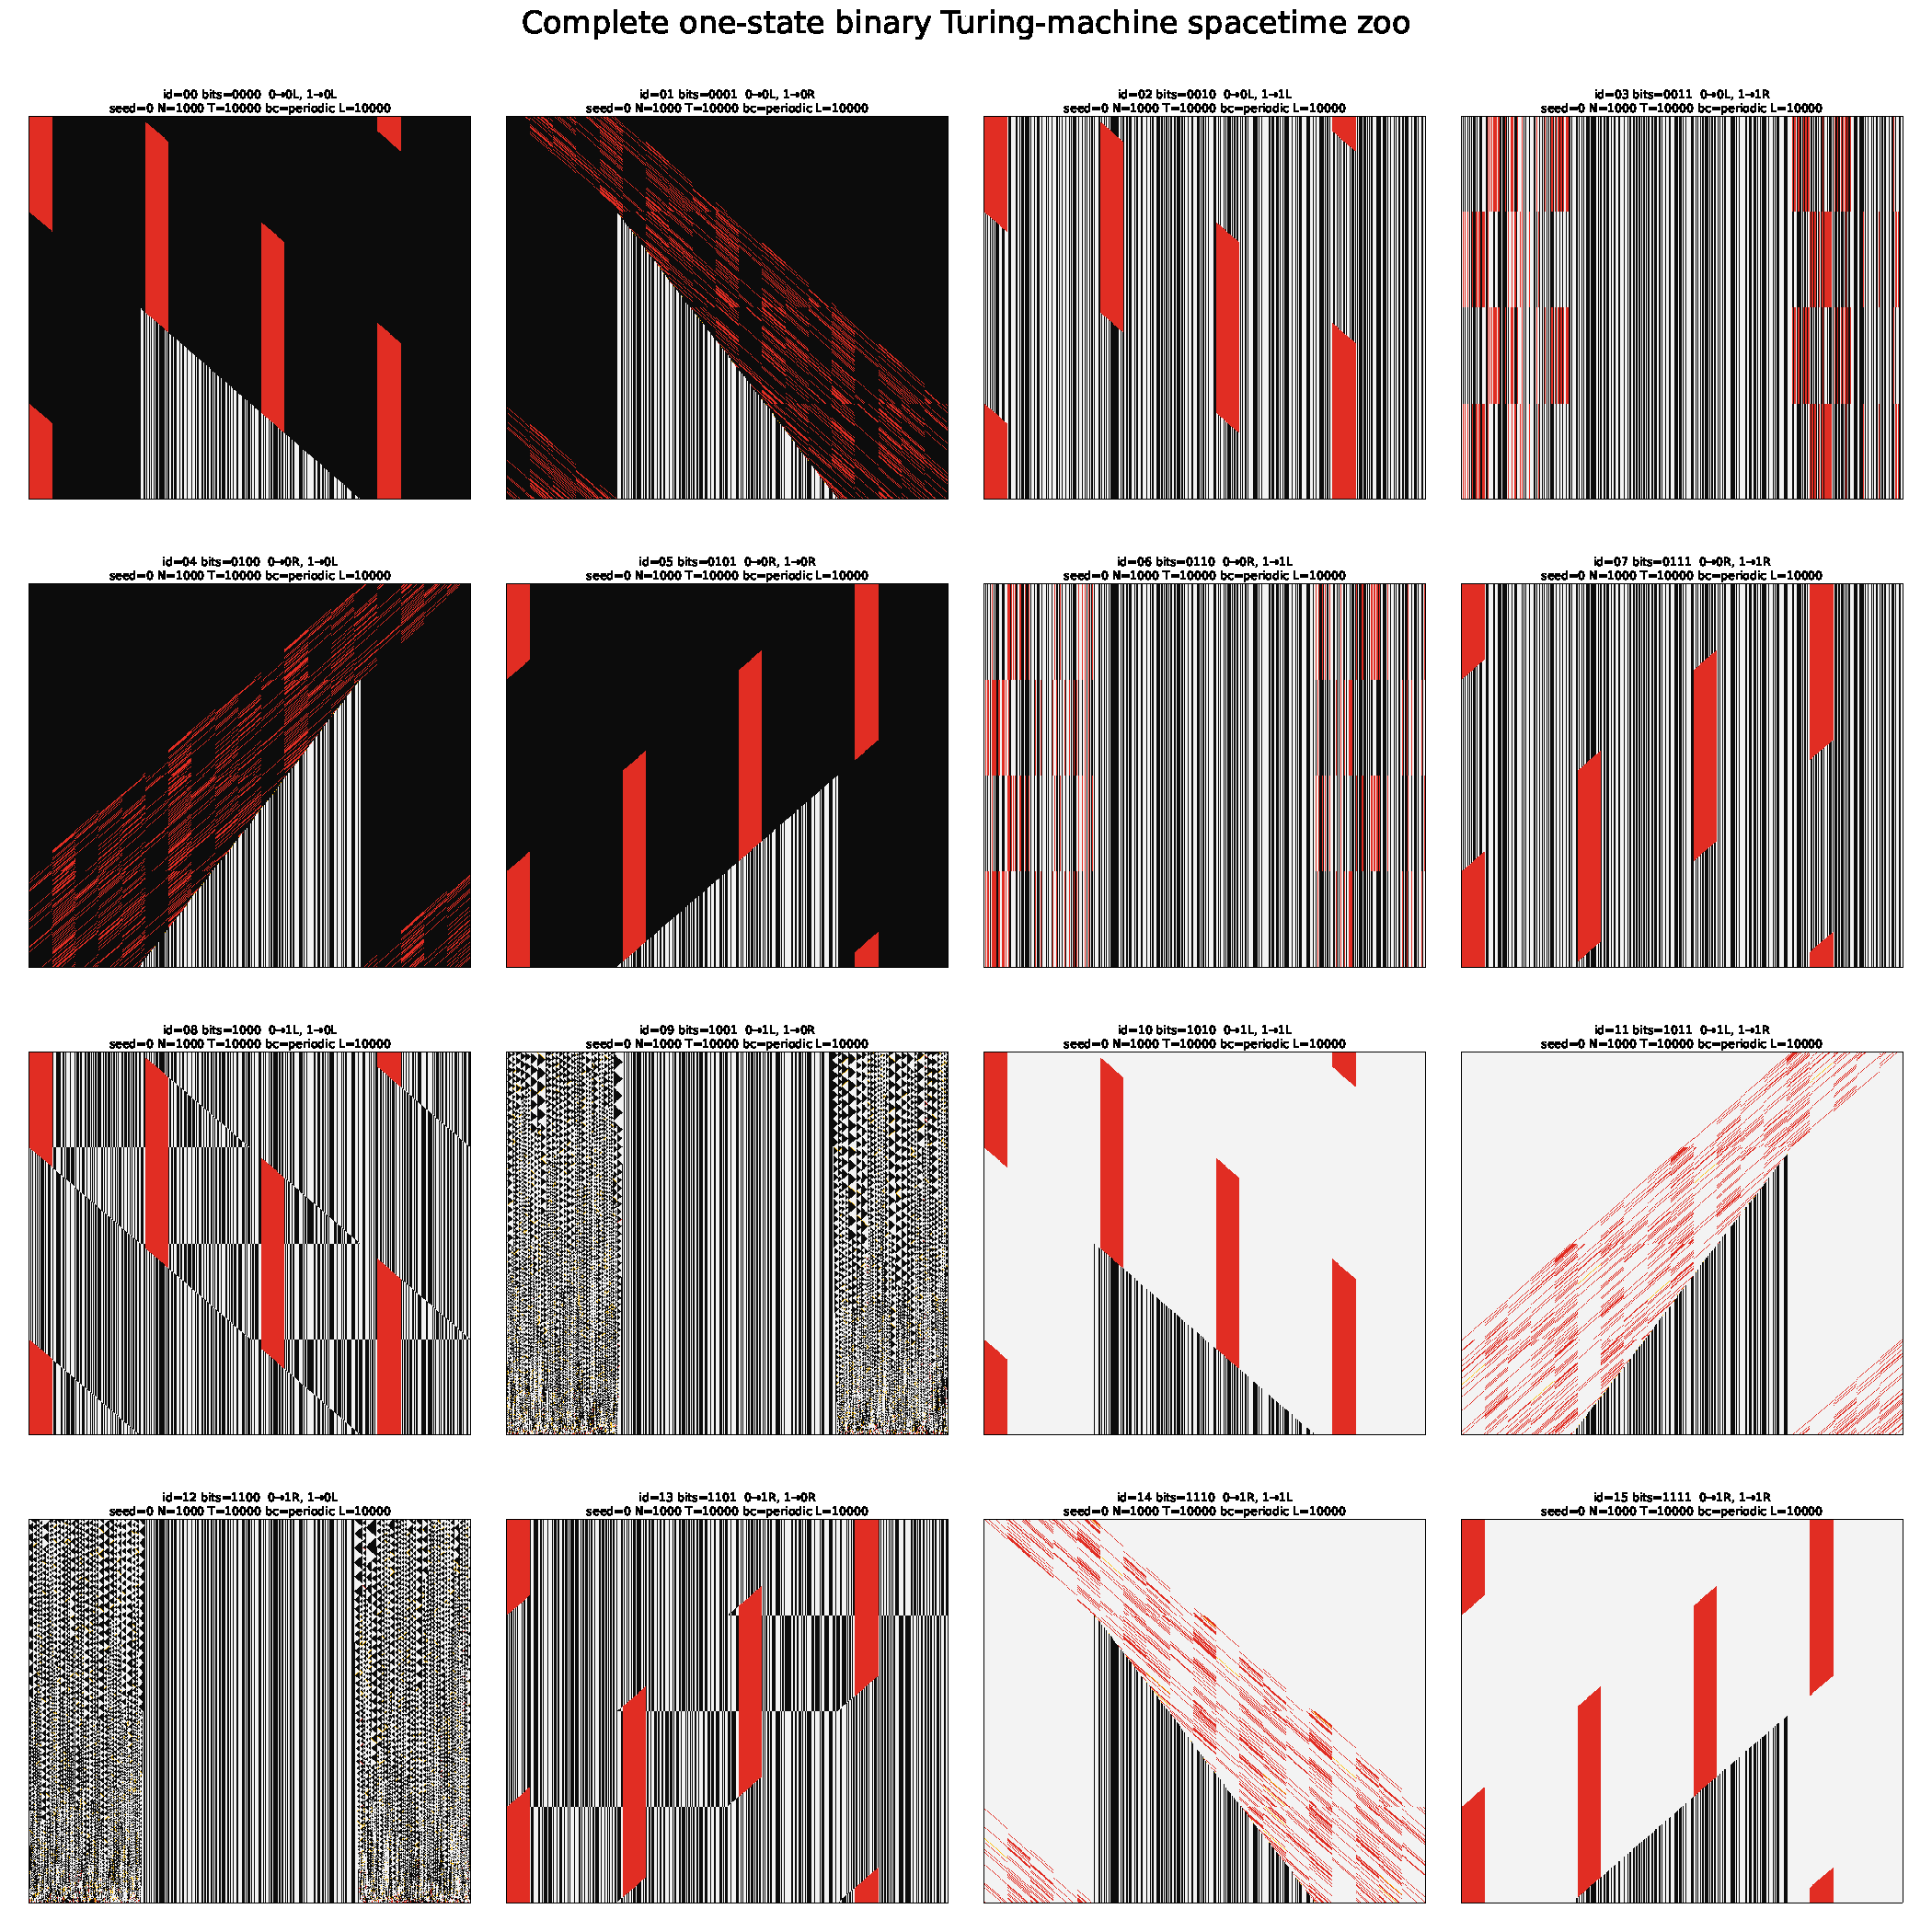
\includegraphics[width=\textwidth]{zoo_tm1_all16.pdf}
\caption{Complete ${\rm TM}_1(2)$ zoo, IDs $0$--$15$ in a $4\times4$ grid.
Each panel uses $N=1000$ identical heads, $q_t^{(i)}=1$, $T=10000$,
$L=10000$ with periodic boundaries, initial spacing five, and the same
Bernoulli-$(1/2)$ tape (seed $0$).  Updates are synchronous; all write
proposals at a site agree.  With $d_b=[M_1(b)+1]/2$, the ID is the binary
word $[W_1(0),d_0,W_1(1),d_1]$, and $S_1(b)=1$.
IDs $0,2,8,10$ move only left and $5,7,13,15$ only right; $3,6$ preserve
the tape and show localized motion here.  IDs $1,4,11,14$ write a constant
symbol and show drifting fronts.  IDs $9,12$ flip symbols and move in
opposite directions for the two reads; ID $9$ is the rule in
Section~\ref{sec:langton-ant}.  Time increases upward; dark/light shows
$V=0/1$, with red/yellow marking single/multiple heads.}
\label{fig:zoo-one-state}
\end{figure}

\clearpage
\begin{figure}[p]
\centering
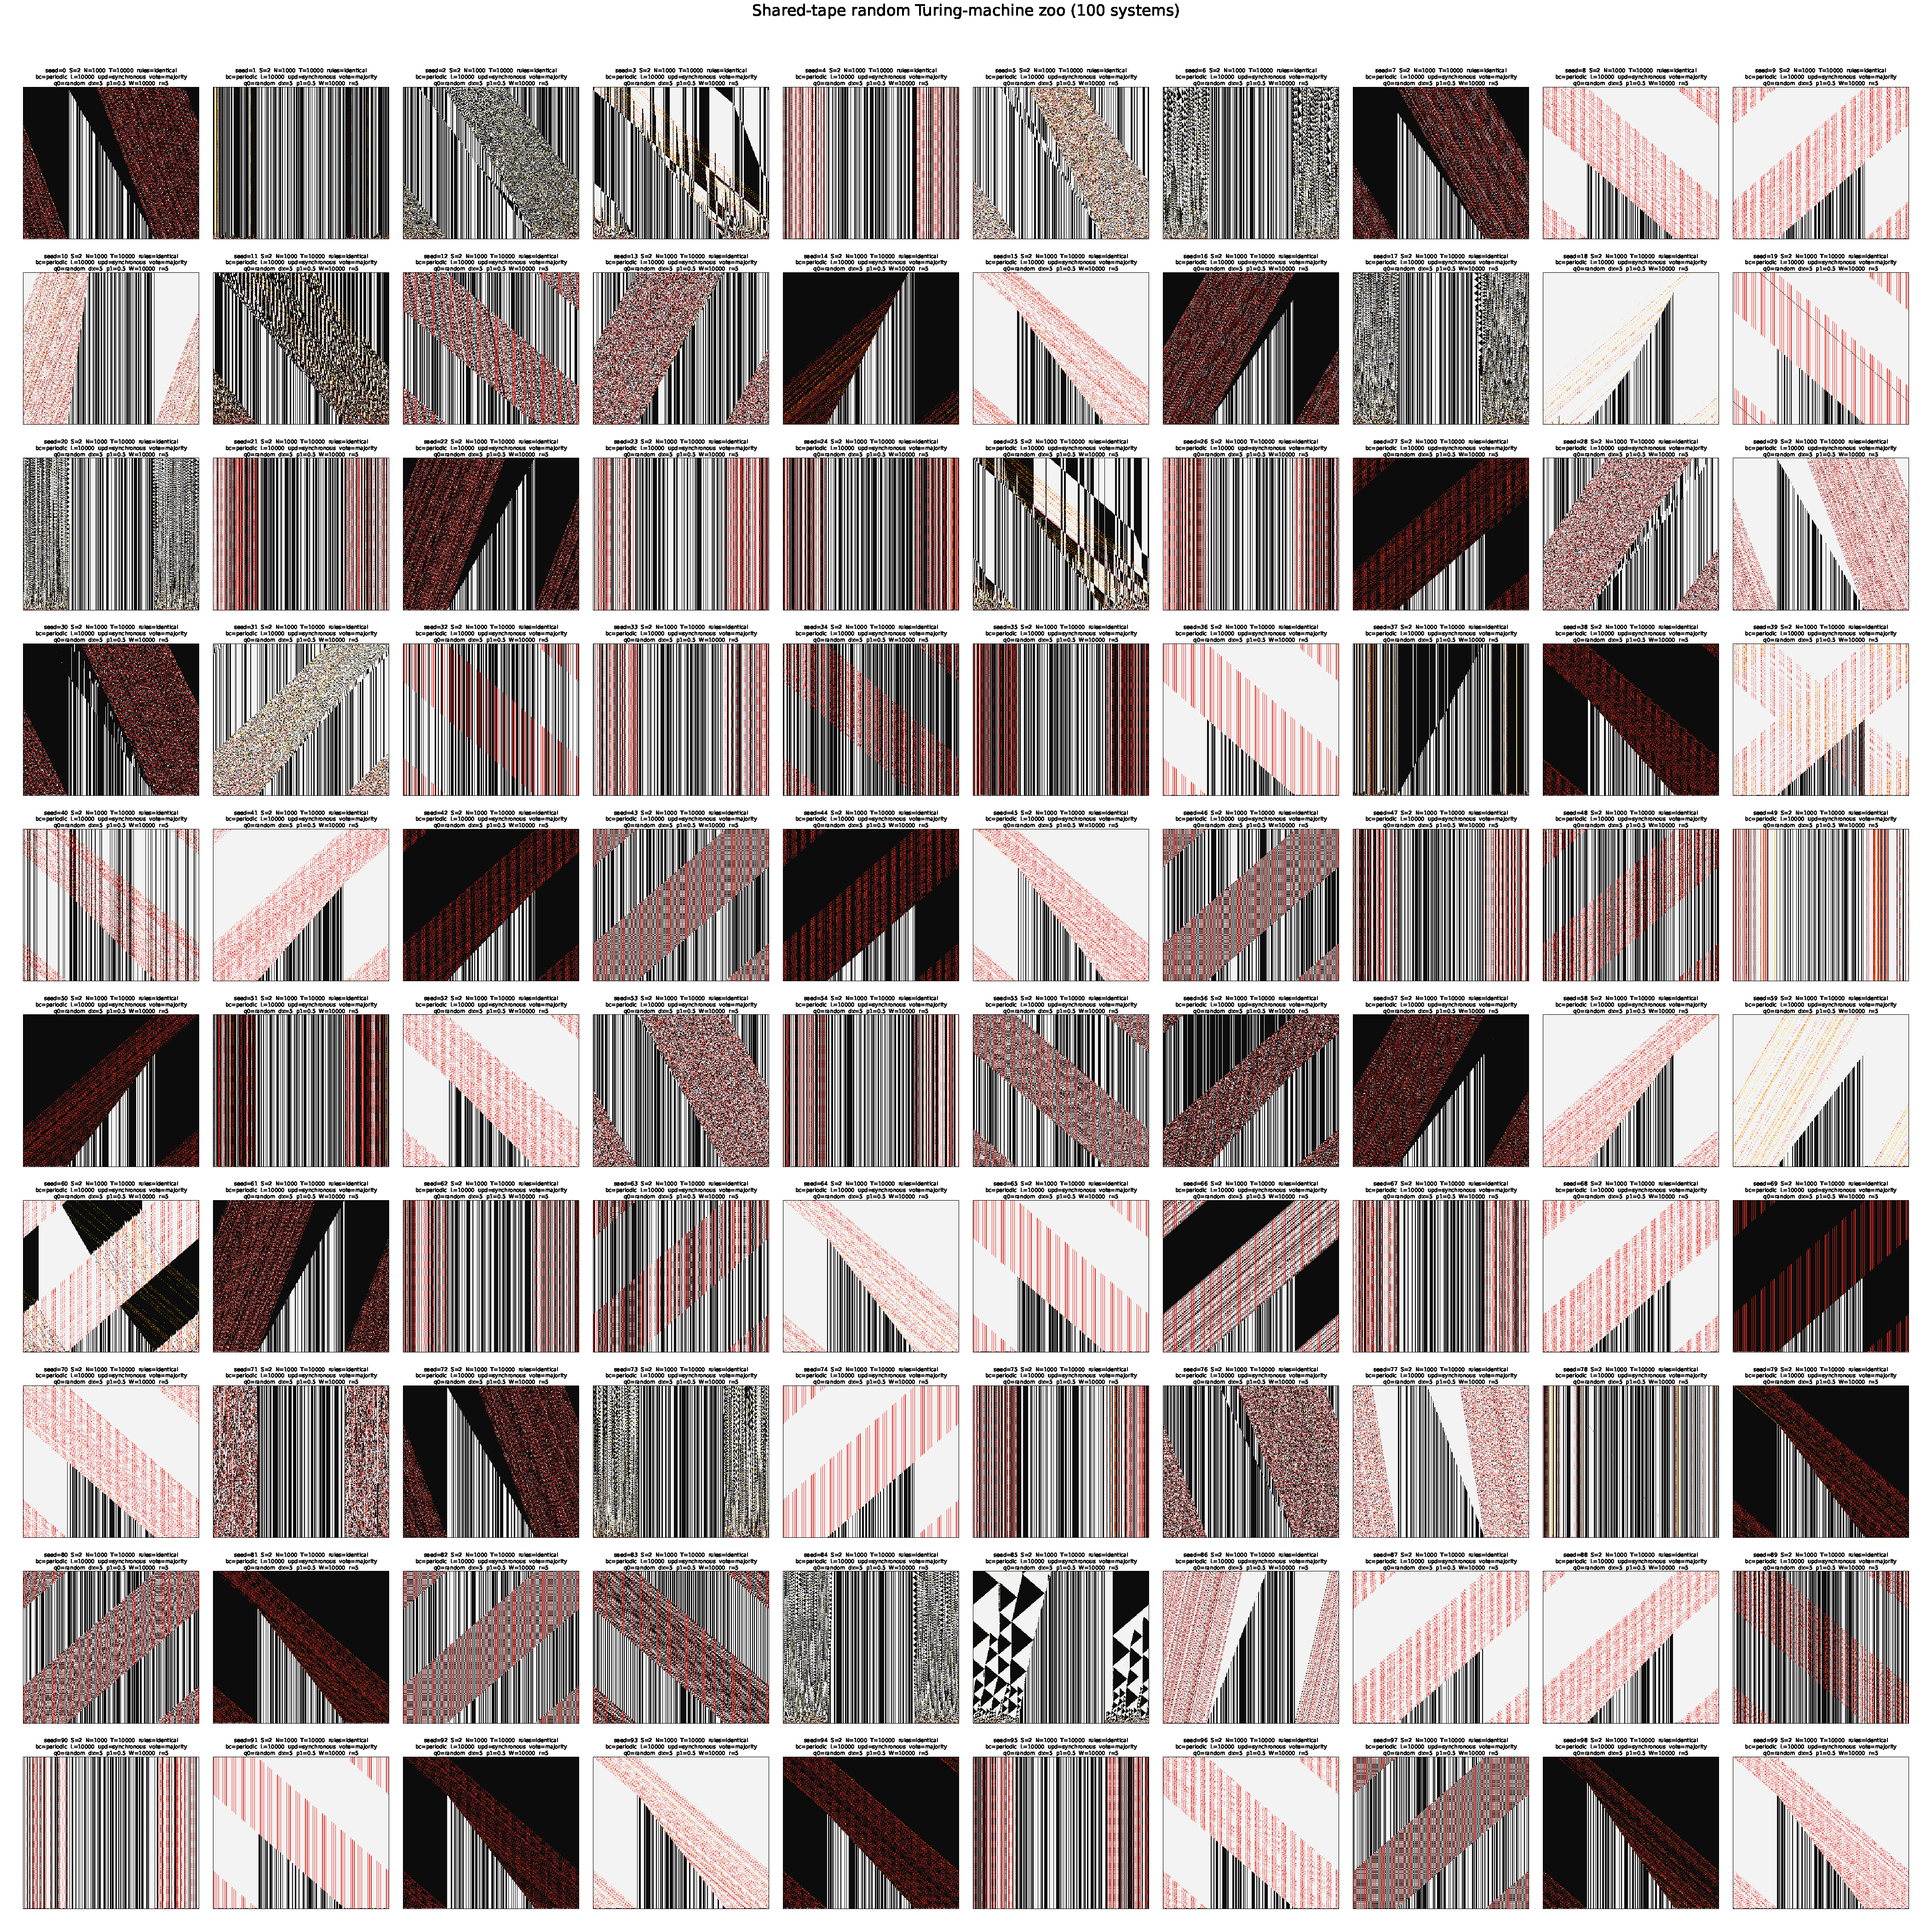
\includegraphics[width=\textwidth]{zoo_tm2_random_states_periodic.pdf}
\caption{Two-state machines with random initial head states.  The 100
panels (seeds $0$--$99$) each contain $N=1000$ copies of one random
${\rm TM}_2(2)$, with $q_0^{(i)}$ uniform on $\{1,2\}$ and a random tape
with $p_1=1/2$.  The ring has $L=10000$, initial head spacing five, and
$T=10000$ synchronous steps with majority-vote writes and unchanged
symbols on ties.  The displayed width equals $L$, and snapshots were
recorded every five steps.  This samples two-state rules rather than
enumerating them; repeated transition tables are possible.  It extends
Fig.~\ref{fig:zoo-one-state} to machines with internal memory.  Time runs
upward; tape values are dark/light and head occupancy is red/yellow.}
\label{fig:zoo-two-state}
\end{figure}

\clearpage
\begin{figure}[p]
\centering
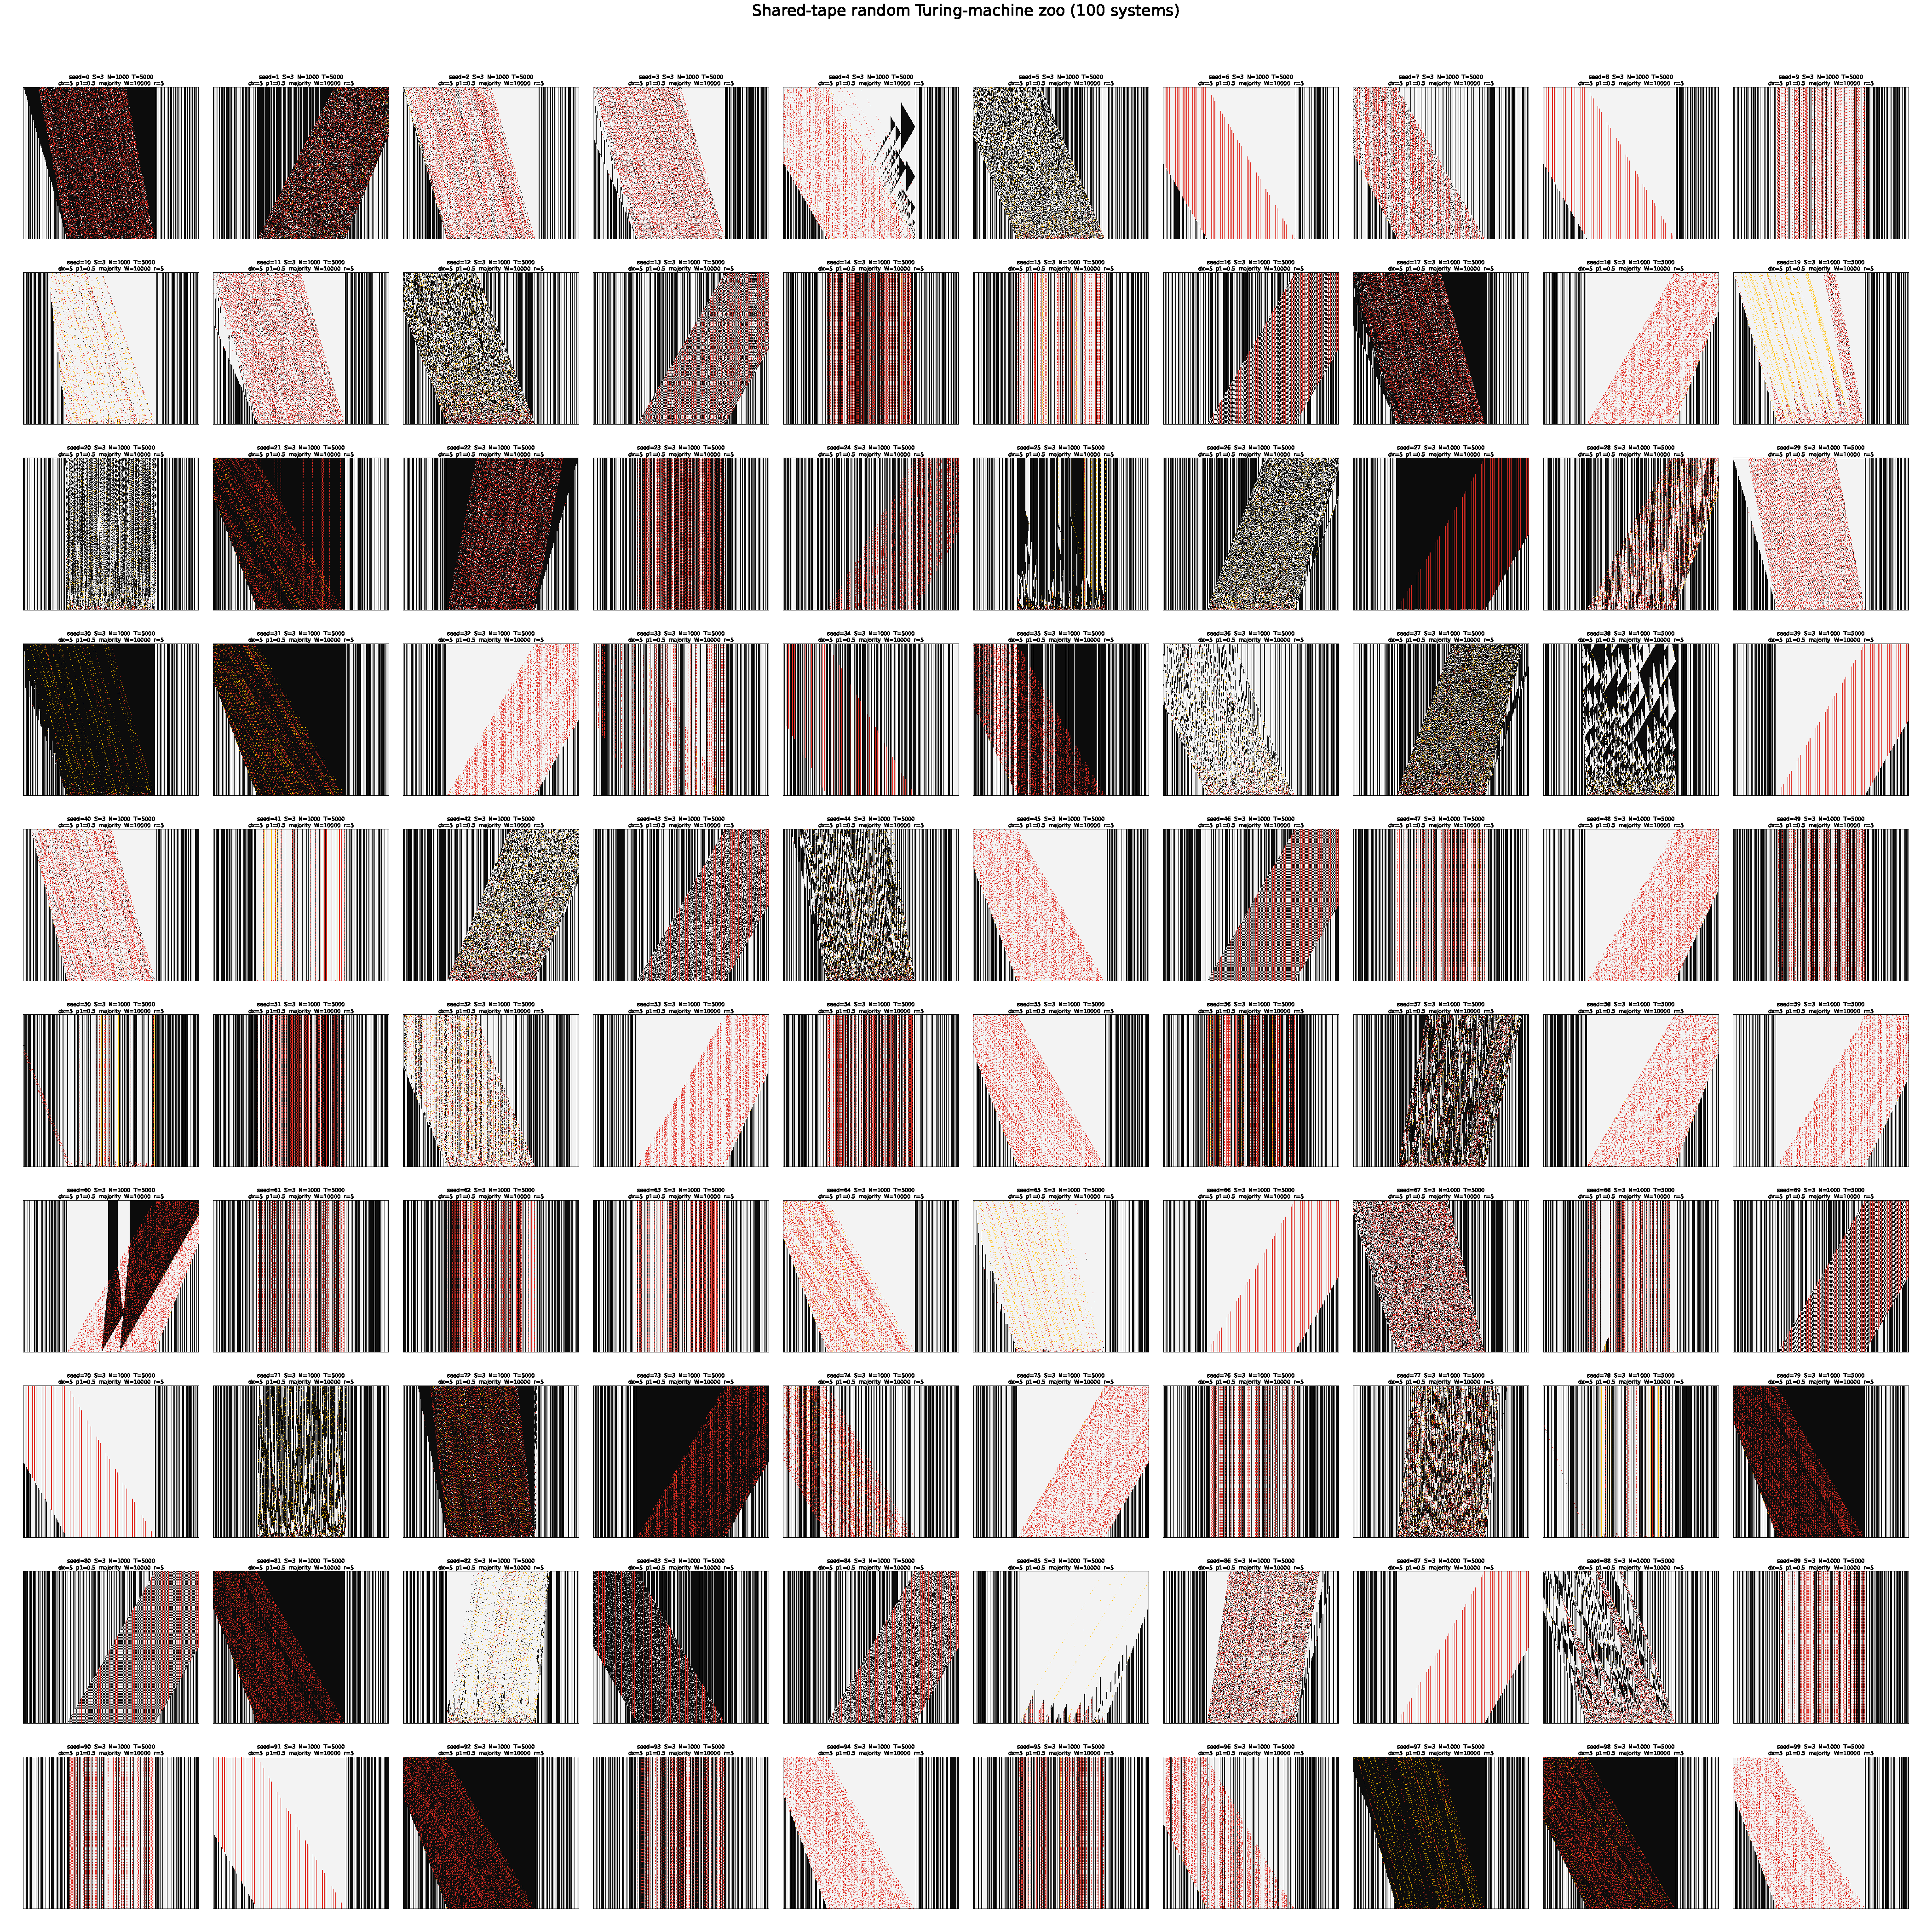
\includegraphics[width=\textwidth]{zoo_tm3_fixed_states.pdf}
\caption{Three-state reference ensemble: 100 random ${\rm TM}_3(2)$
tables, seeds $0$--$99$, with $N=1000$ identical copies per panel and
$q_0^{(i)}=1$.  Each tape starts with independent bits of density
$p_1=1/2$; heads are spaced five sites apart.  Evolution lasts $T=5000$
synchronous steps, with majority-vote writes and unchanged symbols on
ties.  The tape is unbounded and the displayed sites are
$-5000\leq x\leq4999$; leaving the image does not remove a head.
Snapshots were recorded every five steps.  This is the reference for
the additional seeds, blank tape, and asynchronous comparisons below.
Time runs upward; dark/light denotes $V=0/1$, and red/yellow denotes
single/multiple heads.}
\label{fig:zoo-three-state}
\end{figure}

\clearpage
\begin{figure}[p]
\centering
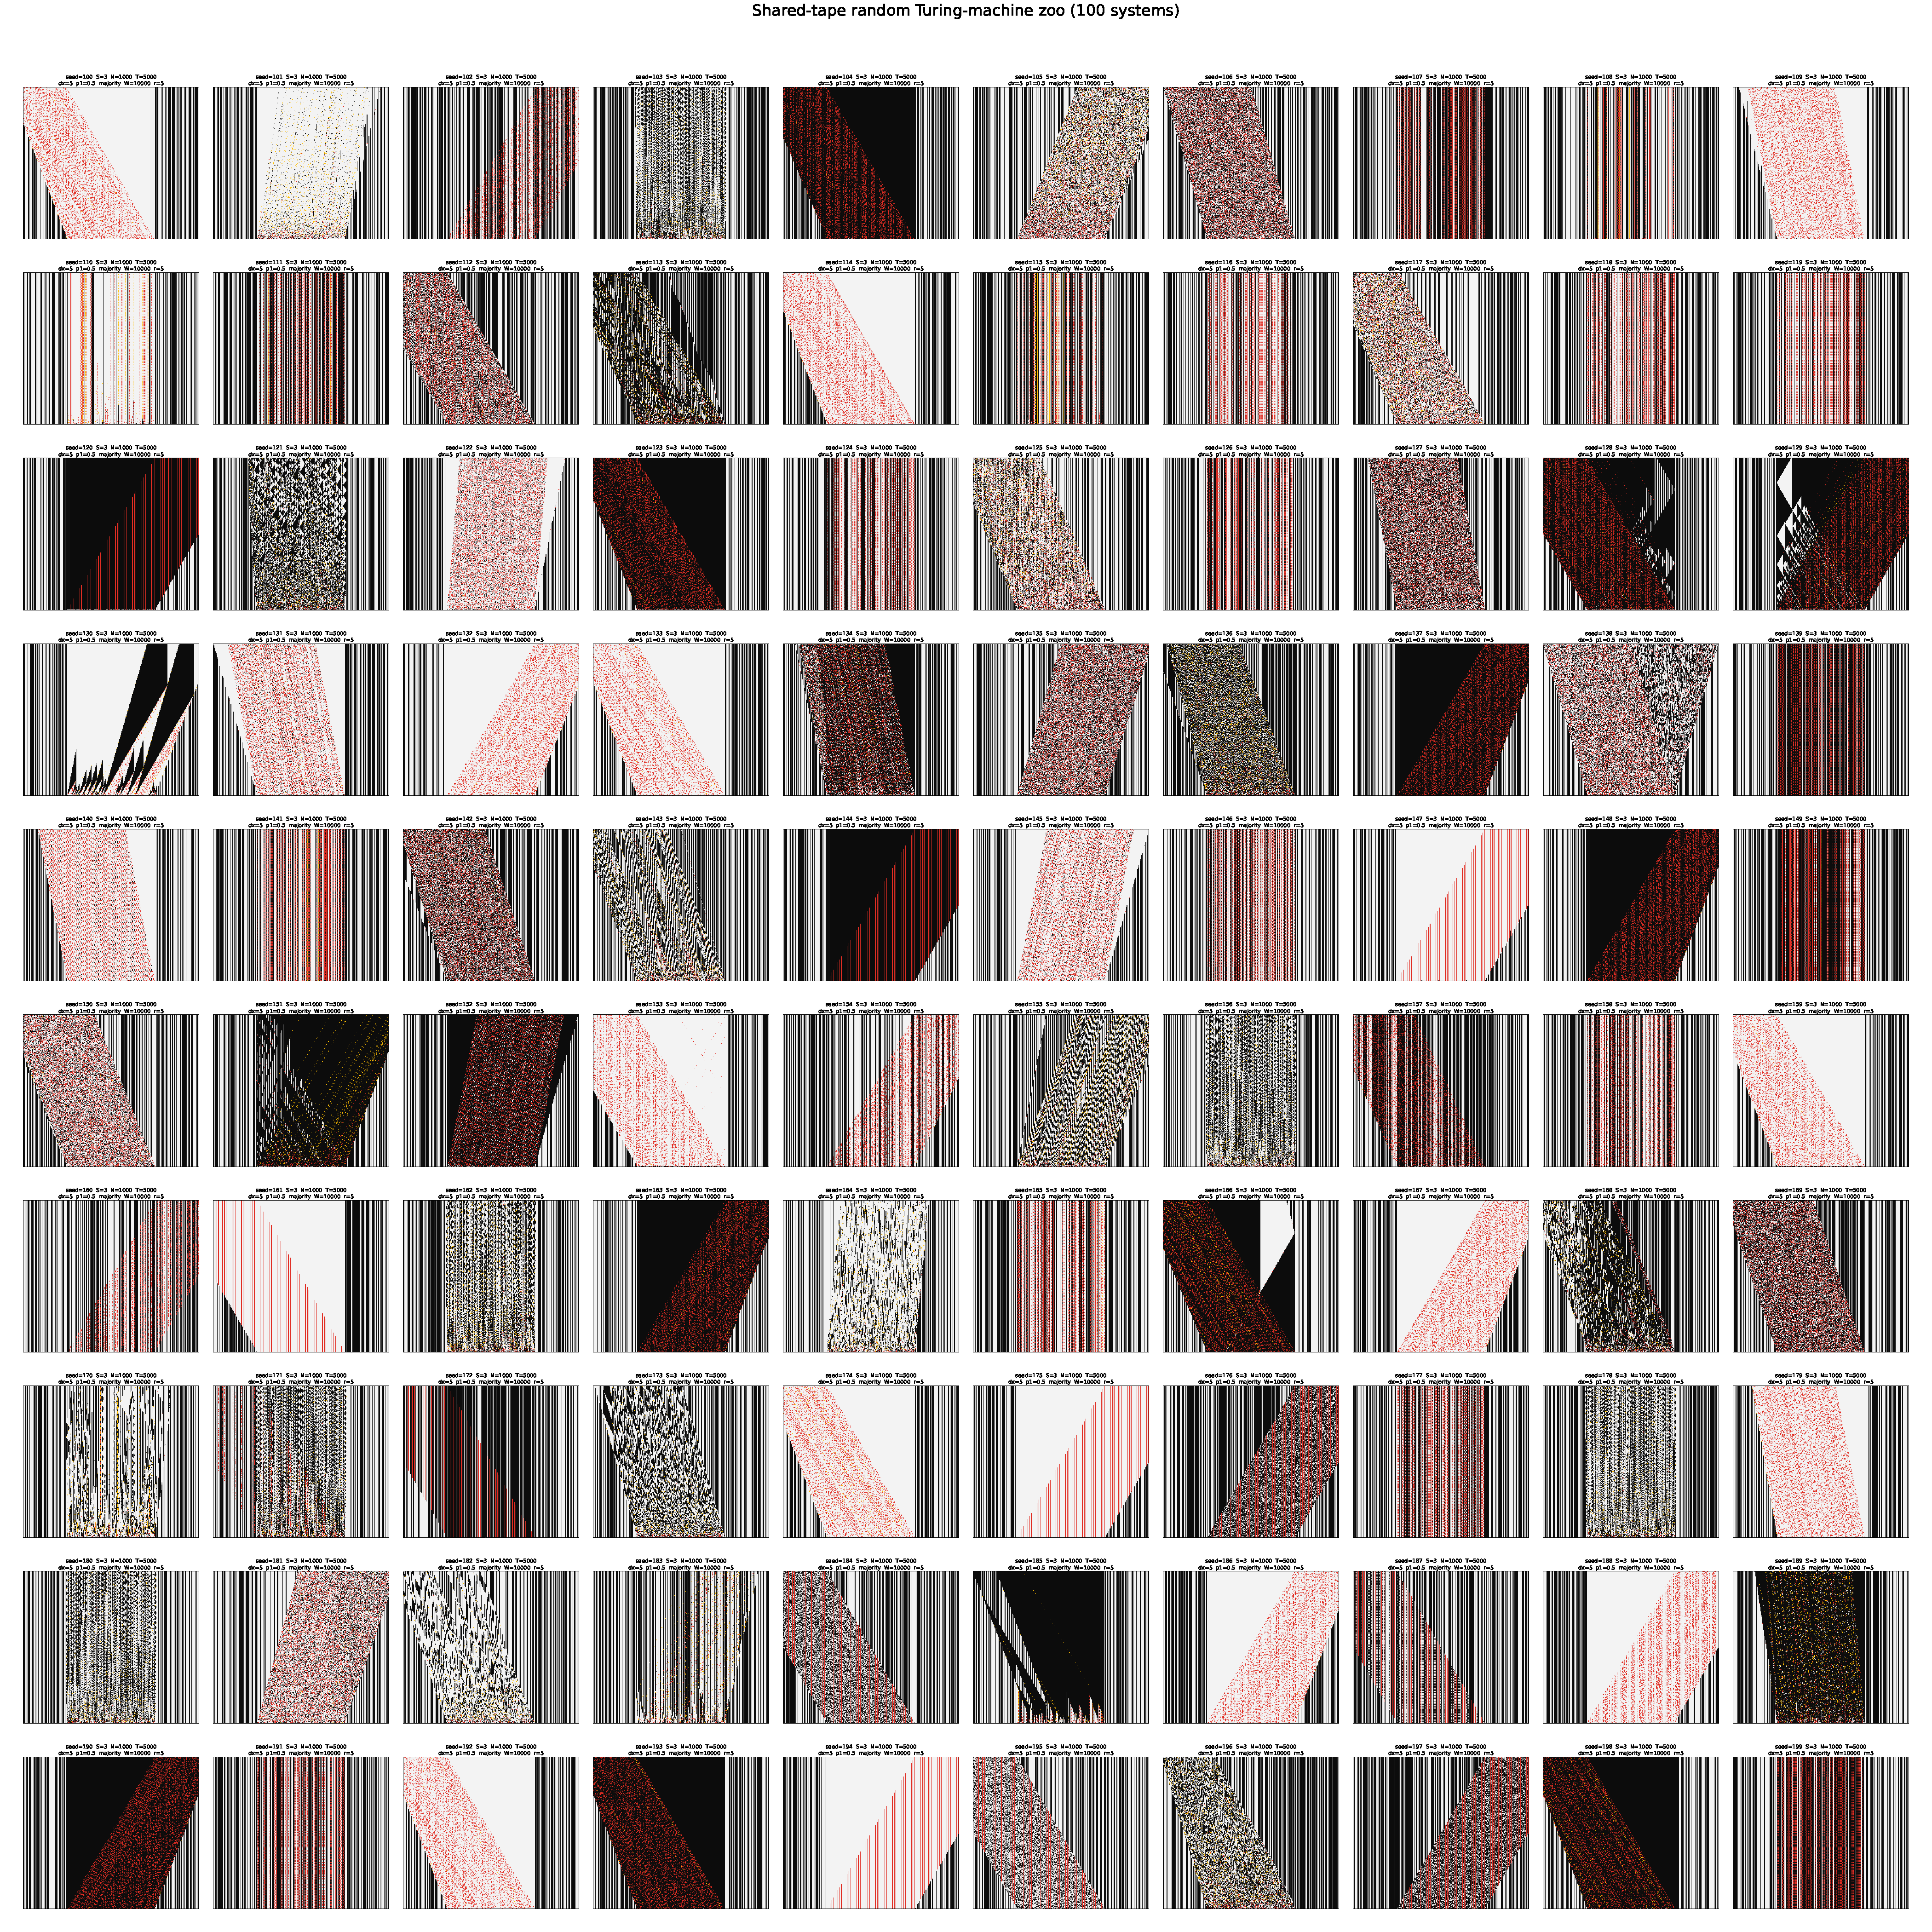
\includegraphics[width=\textwidth]{zoo_tm3_seeds100-199.pdf}
\caption{A second sample of the three-state reference ensemble, using
seeds $100$--$199$ in reading order.  Each of the 100 panels contains
$N=1000$ identical copies of a random ${\rm TM}_3(2)$, initialized at
$q_0^{(i)}=1$ on a Bernoulli-$(1/2)$ tape with head spacing five.
The $T=5000$ updates are synchronous, with majority-vote writes and
unchanged symbols on ties; the unbounded tape is displayed over
$-5000\leq x\leq4999$, with snapshots recorded every five steps.
All ensemble parameters match Fig.~\ref{fig:zoo-three-state}; the new
seeds broaden the sample of tables and initial tapes, rather than
continuing the earlier trajectories.  Time runs upward, with the same
tape and occupancy colors.}
\label{fig:zoo-three-more}
\end{figure}

\clearpage
\begin{figure}[p]
\centering
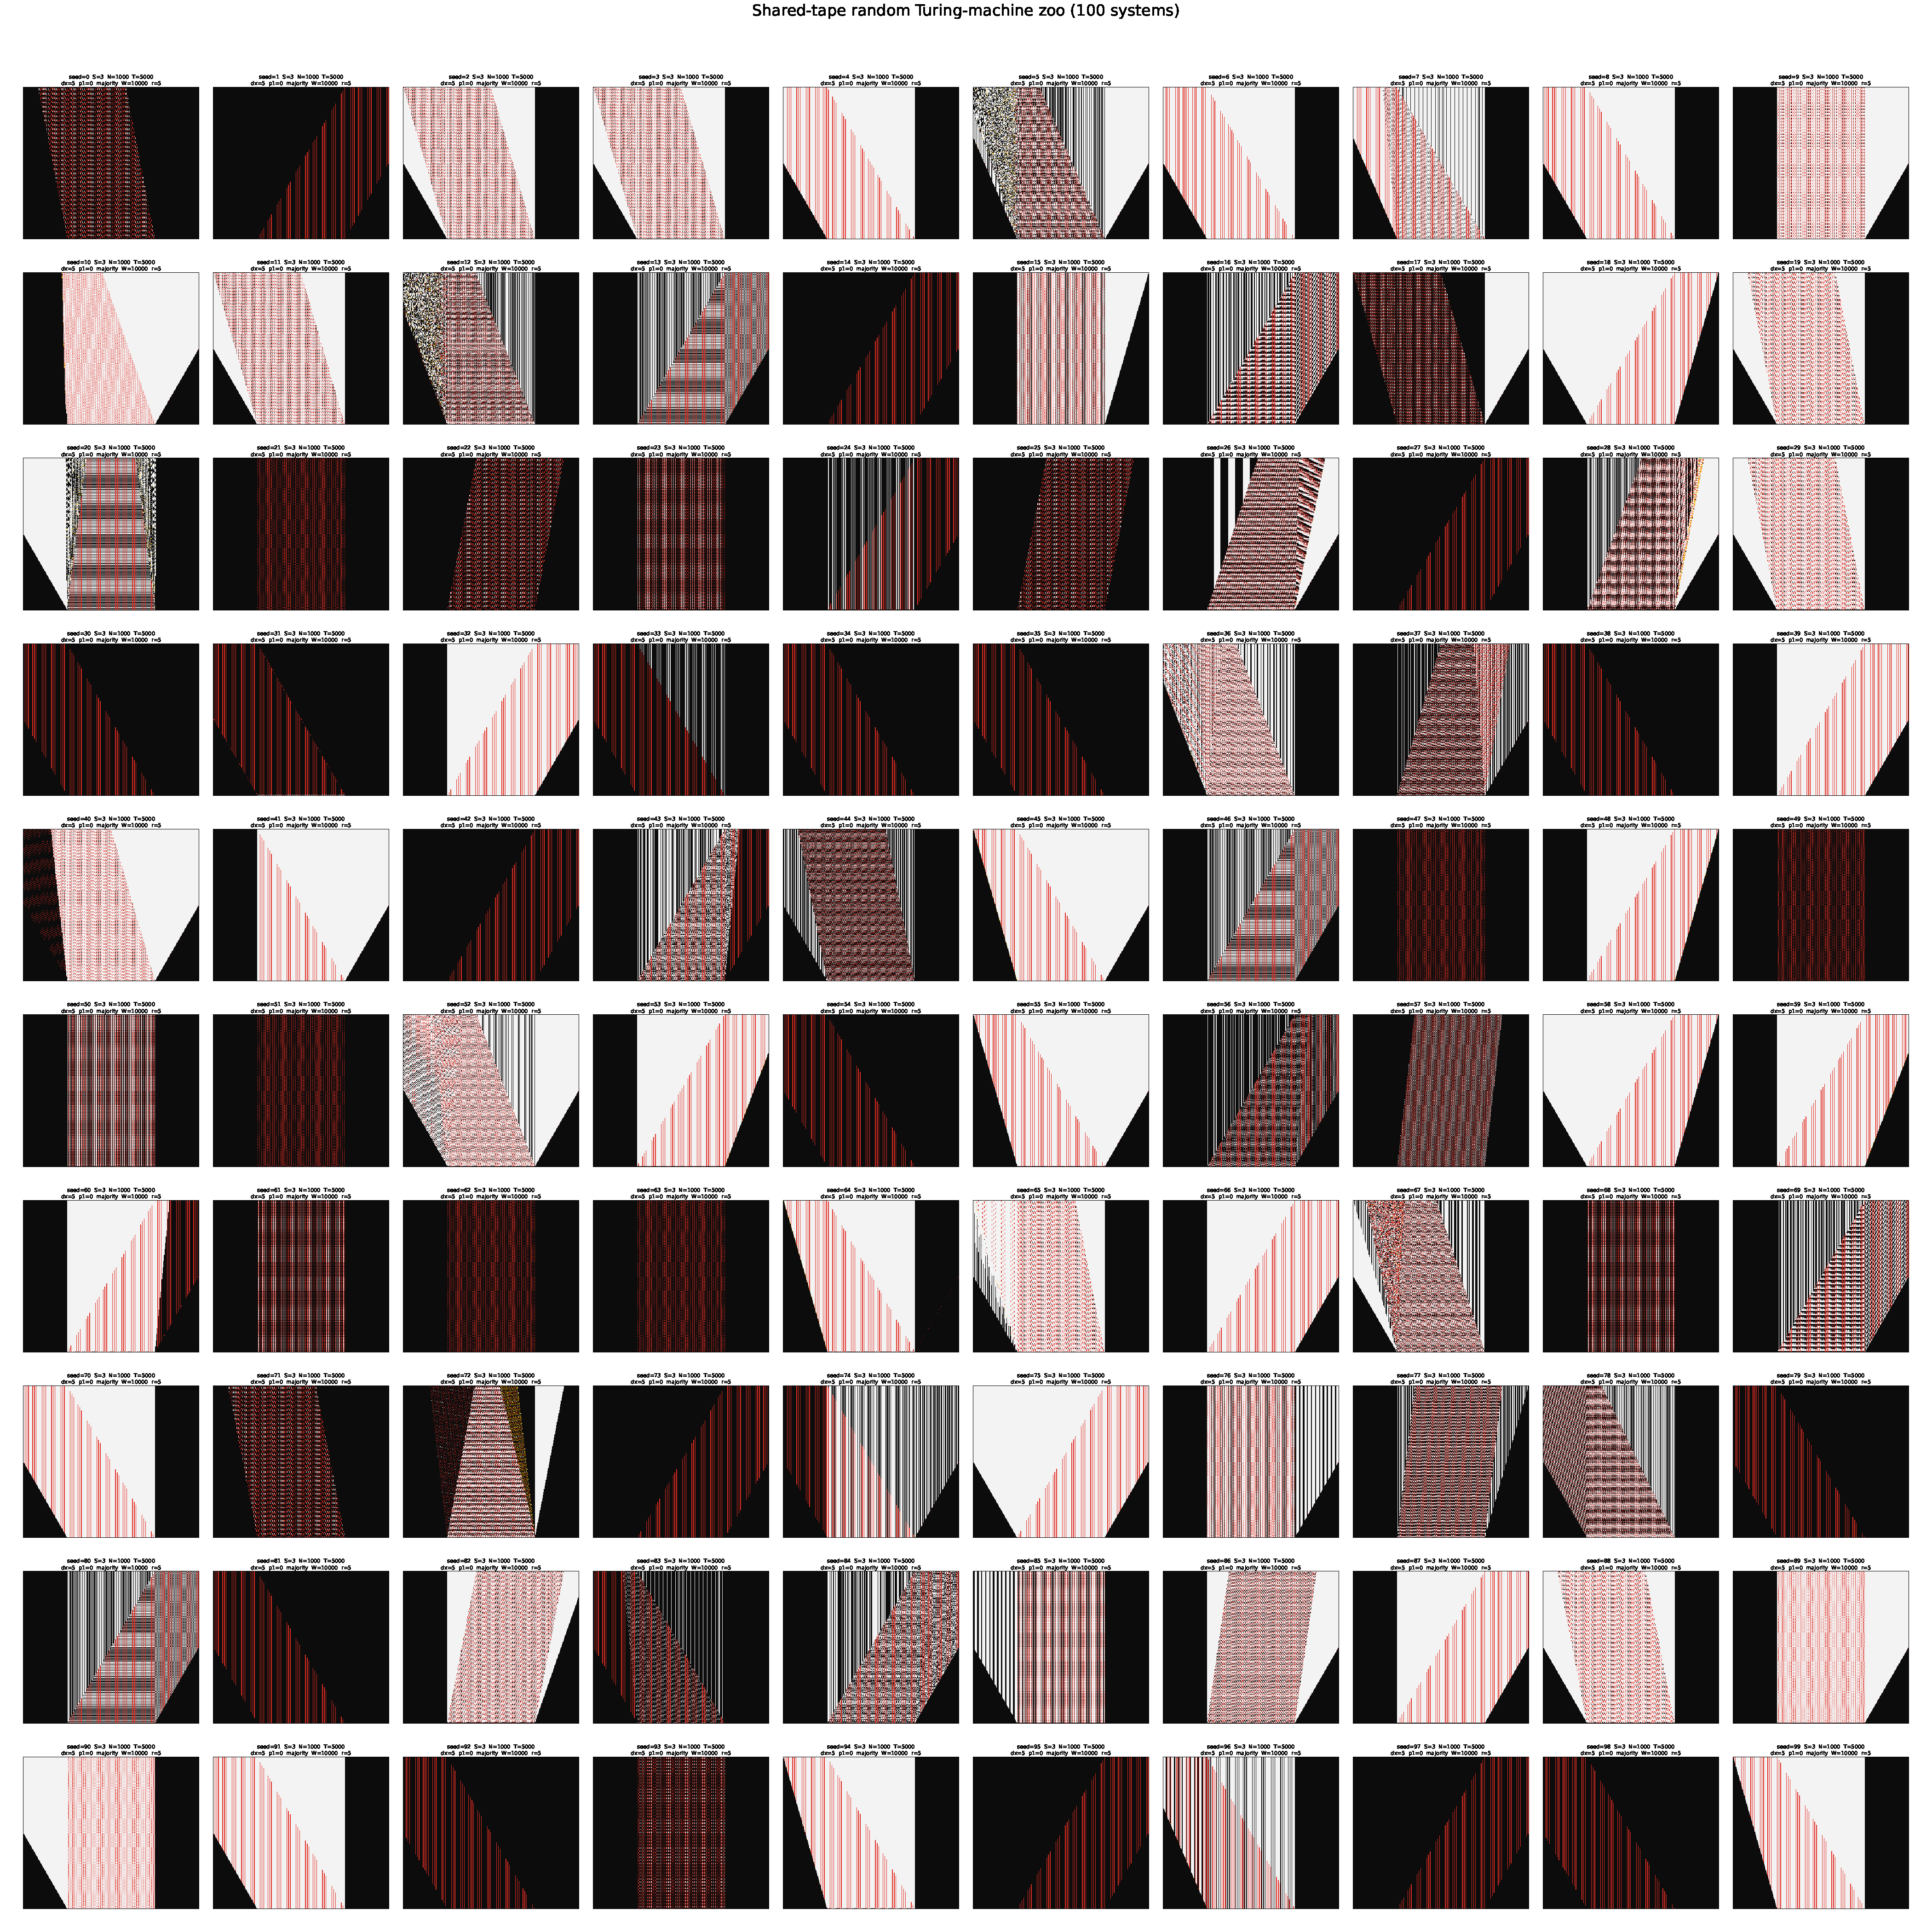
\includegraphics[width=\textwidth]{zoo_tm3_blank_tape.pdf}
\caption{Three-state machines on a blank tape, $V_0(x)=0$.  Seeds
$0$--$99$ use exactly the same ${\rm TM}_3(2)$ tables as
Fig.~\ref{fig:zoo-three-state}, with $N=1000$ identical heads per panel,
$q_0^{(i)}=1$, and initial spacing five.  The runs have $T=5000$
synchronous steps, majority-vote writes with unchanged symbols on ties,
and an unbounded tape displayed over $-5000\leq x\leq4999$.
Snapshots were recorded every five steps.  This comparison changes the
initial landscape while retaining the transition tables; the blank
background also makes regions modified by passing heads conspicuous.
Time increases upward.  Dark/light shows $V=0/1$, and red/yellow shows
single/multiple heads, not internal states.}
\label{fig:zoo-three-blank}
\end{figure}

\clearpage
\begin{figure}[p]
\centering
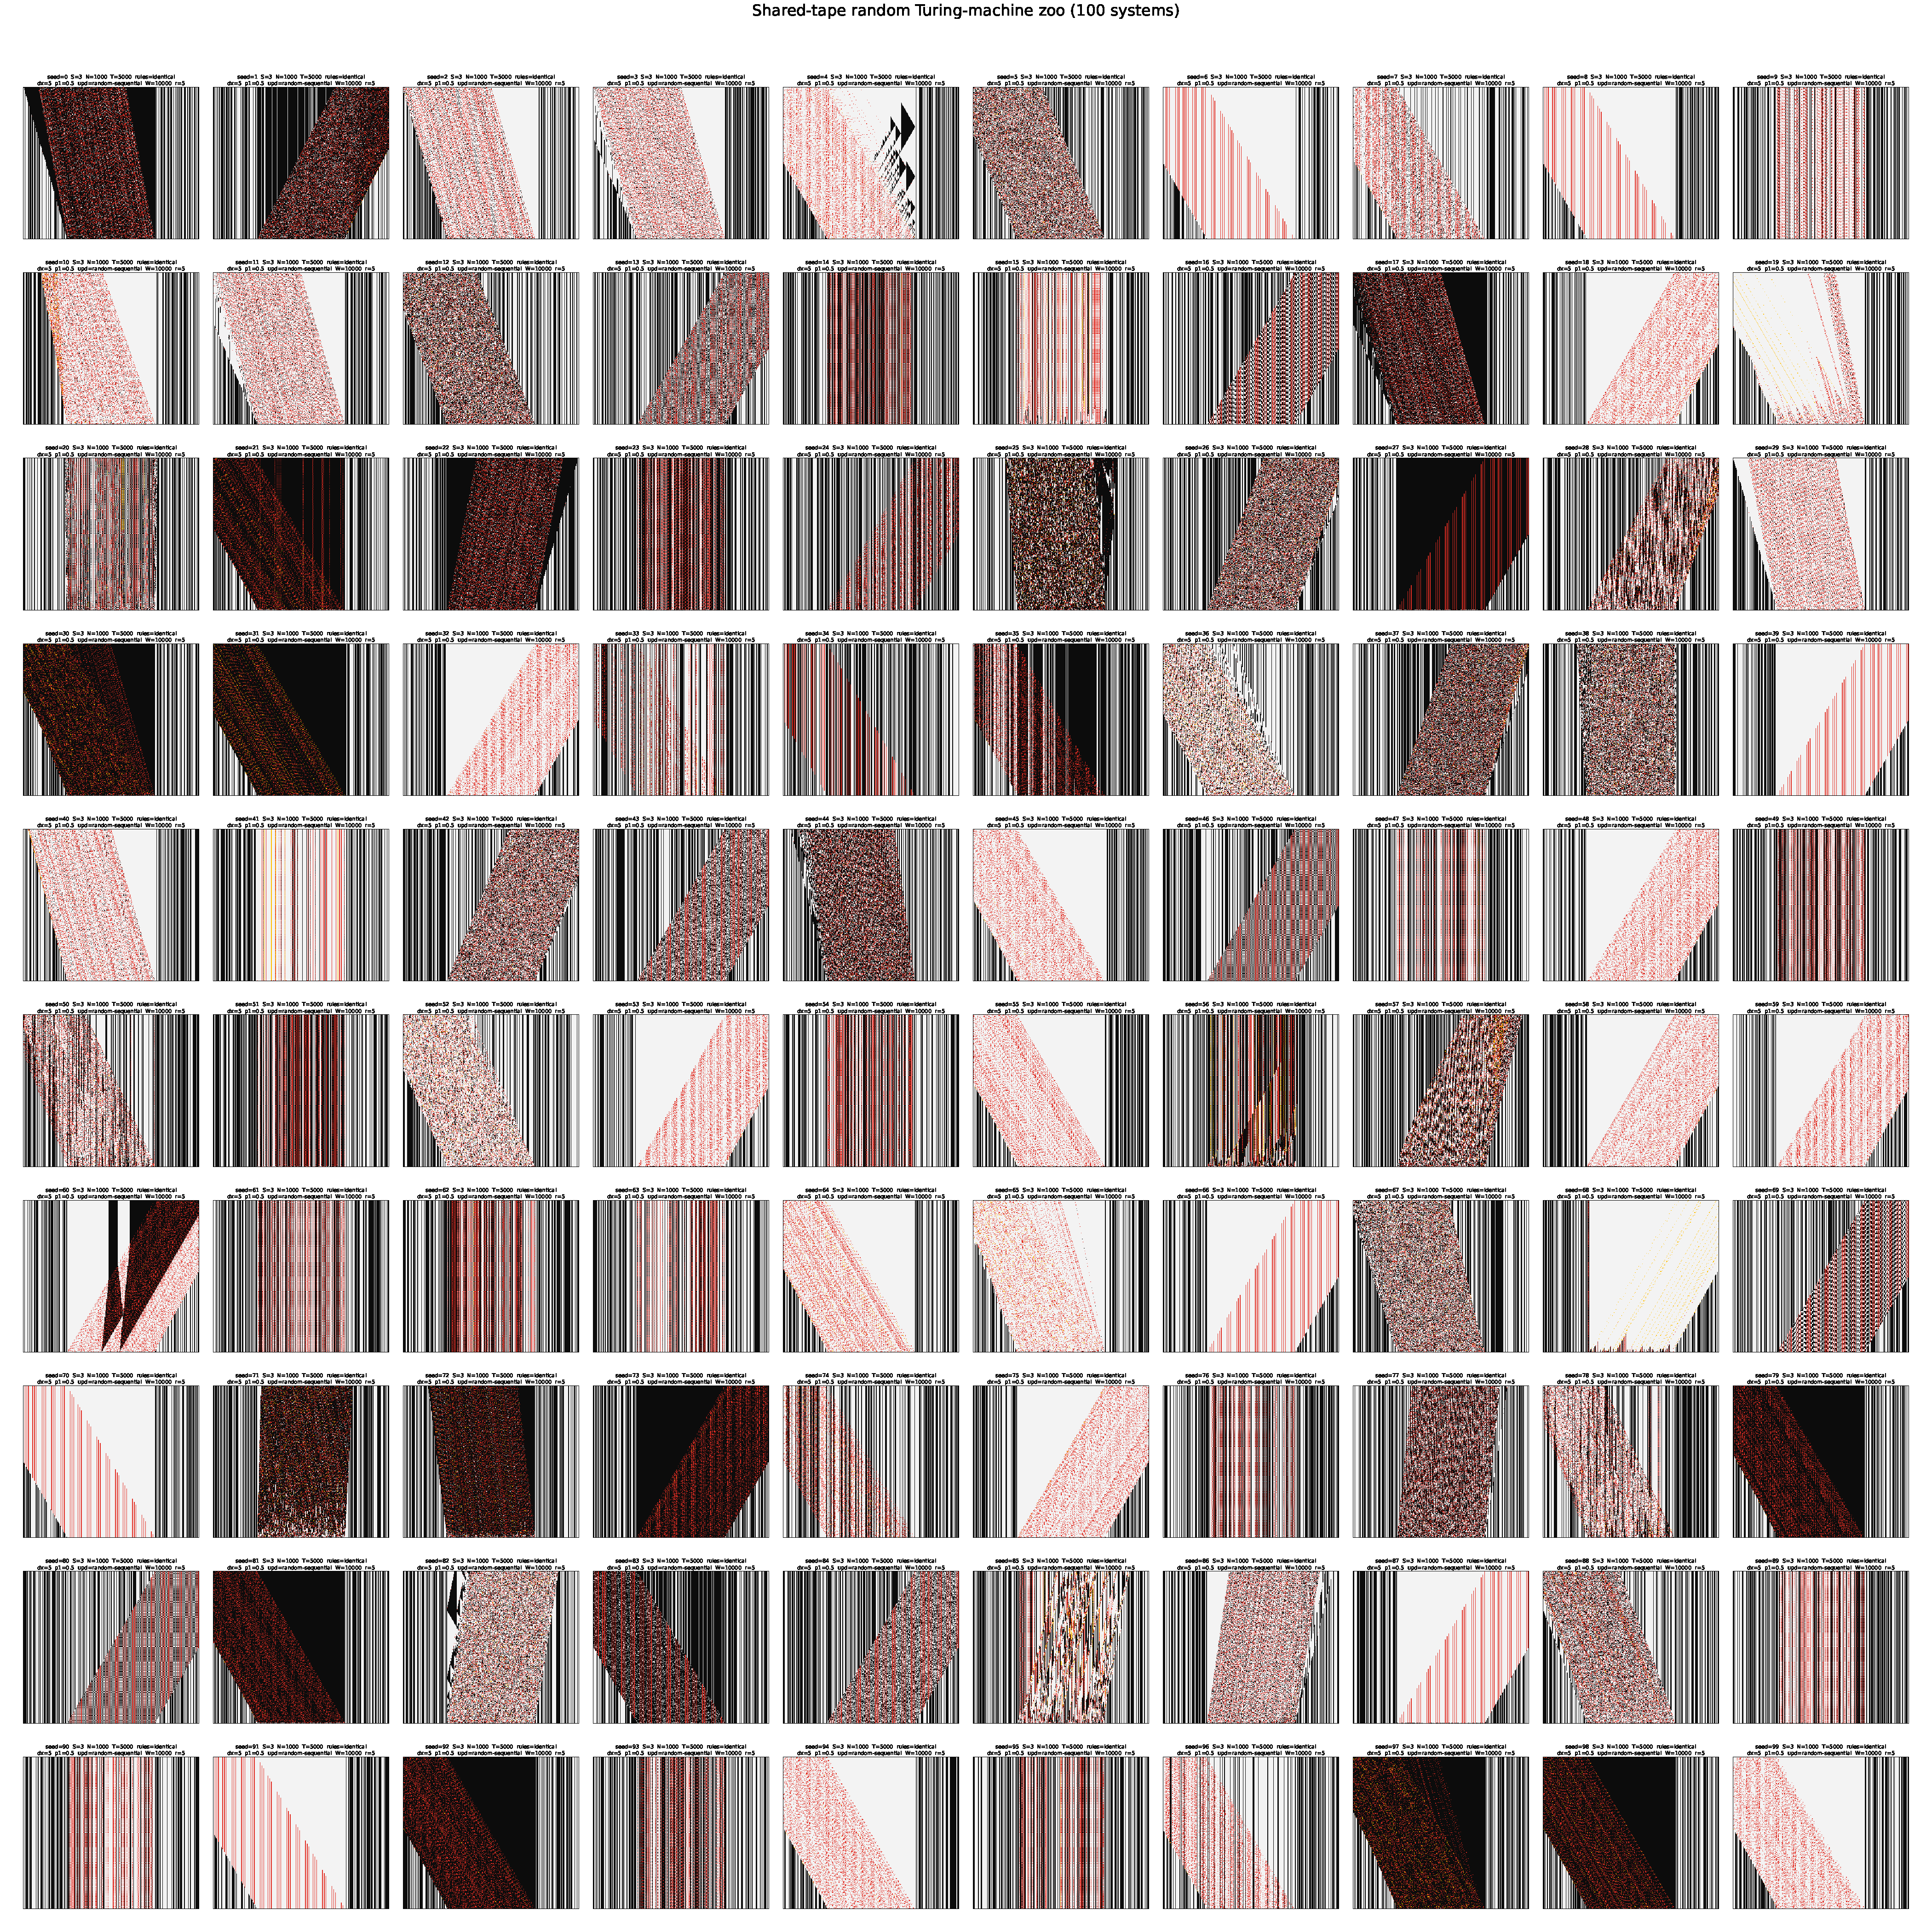
\includegraphics[width=\textwidth]{zoo_tm3_async.pdf}
\caption{Random-sequential evolution of identical ${\rm TM}_3(2)$
agents.  The 100 panels, seeds $0$--$99$, use the same transition tables
as Fig.~\ref{fig:zoo-three-state}, with $N=1000$, $q_0^{(i)}=1$,
$p_1=1/2$, and initial spacing five.  Here $T=5000$ counts sweeps, each
updating every head once in a fresh random order; writes take effect
immediately, so majority voting is not applied.  The tape is unbounded,
the display covers $-5000\leq x\leq4999$, and snapshots were recorded
every five sweeps.  The comparison tests sensitivity to update order
while preserving the individual machine rules.  Time increases upward;
the red/yellow overlay records occupancy at sweep boundaries and does
not display the intermediate actions within a sweep.}
\label{fig:zoo-three-async}
\end{figure}

\clearpage
\begin{figure}[p]
\centering
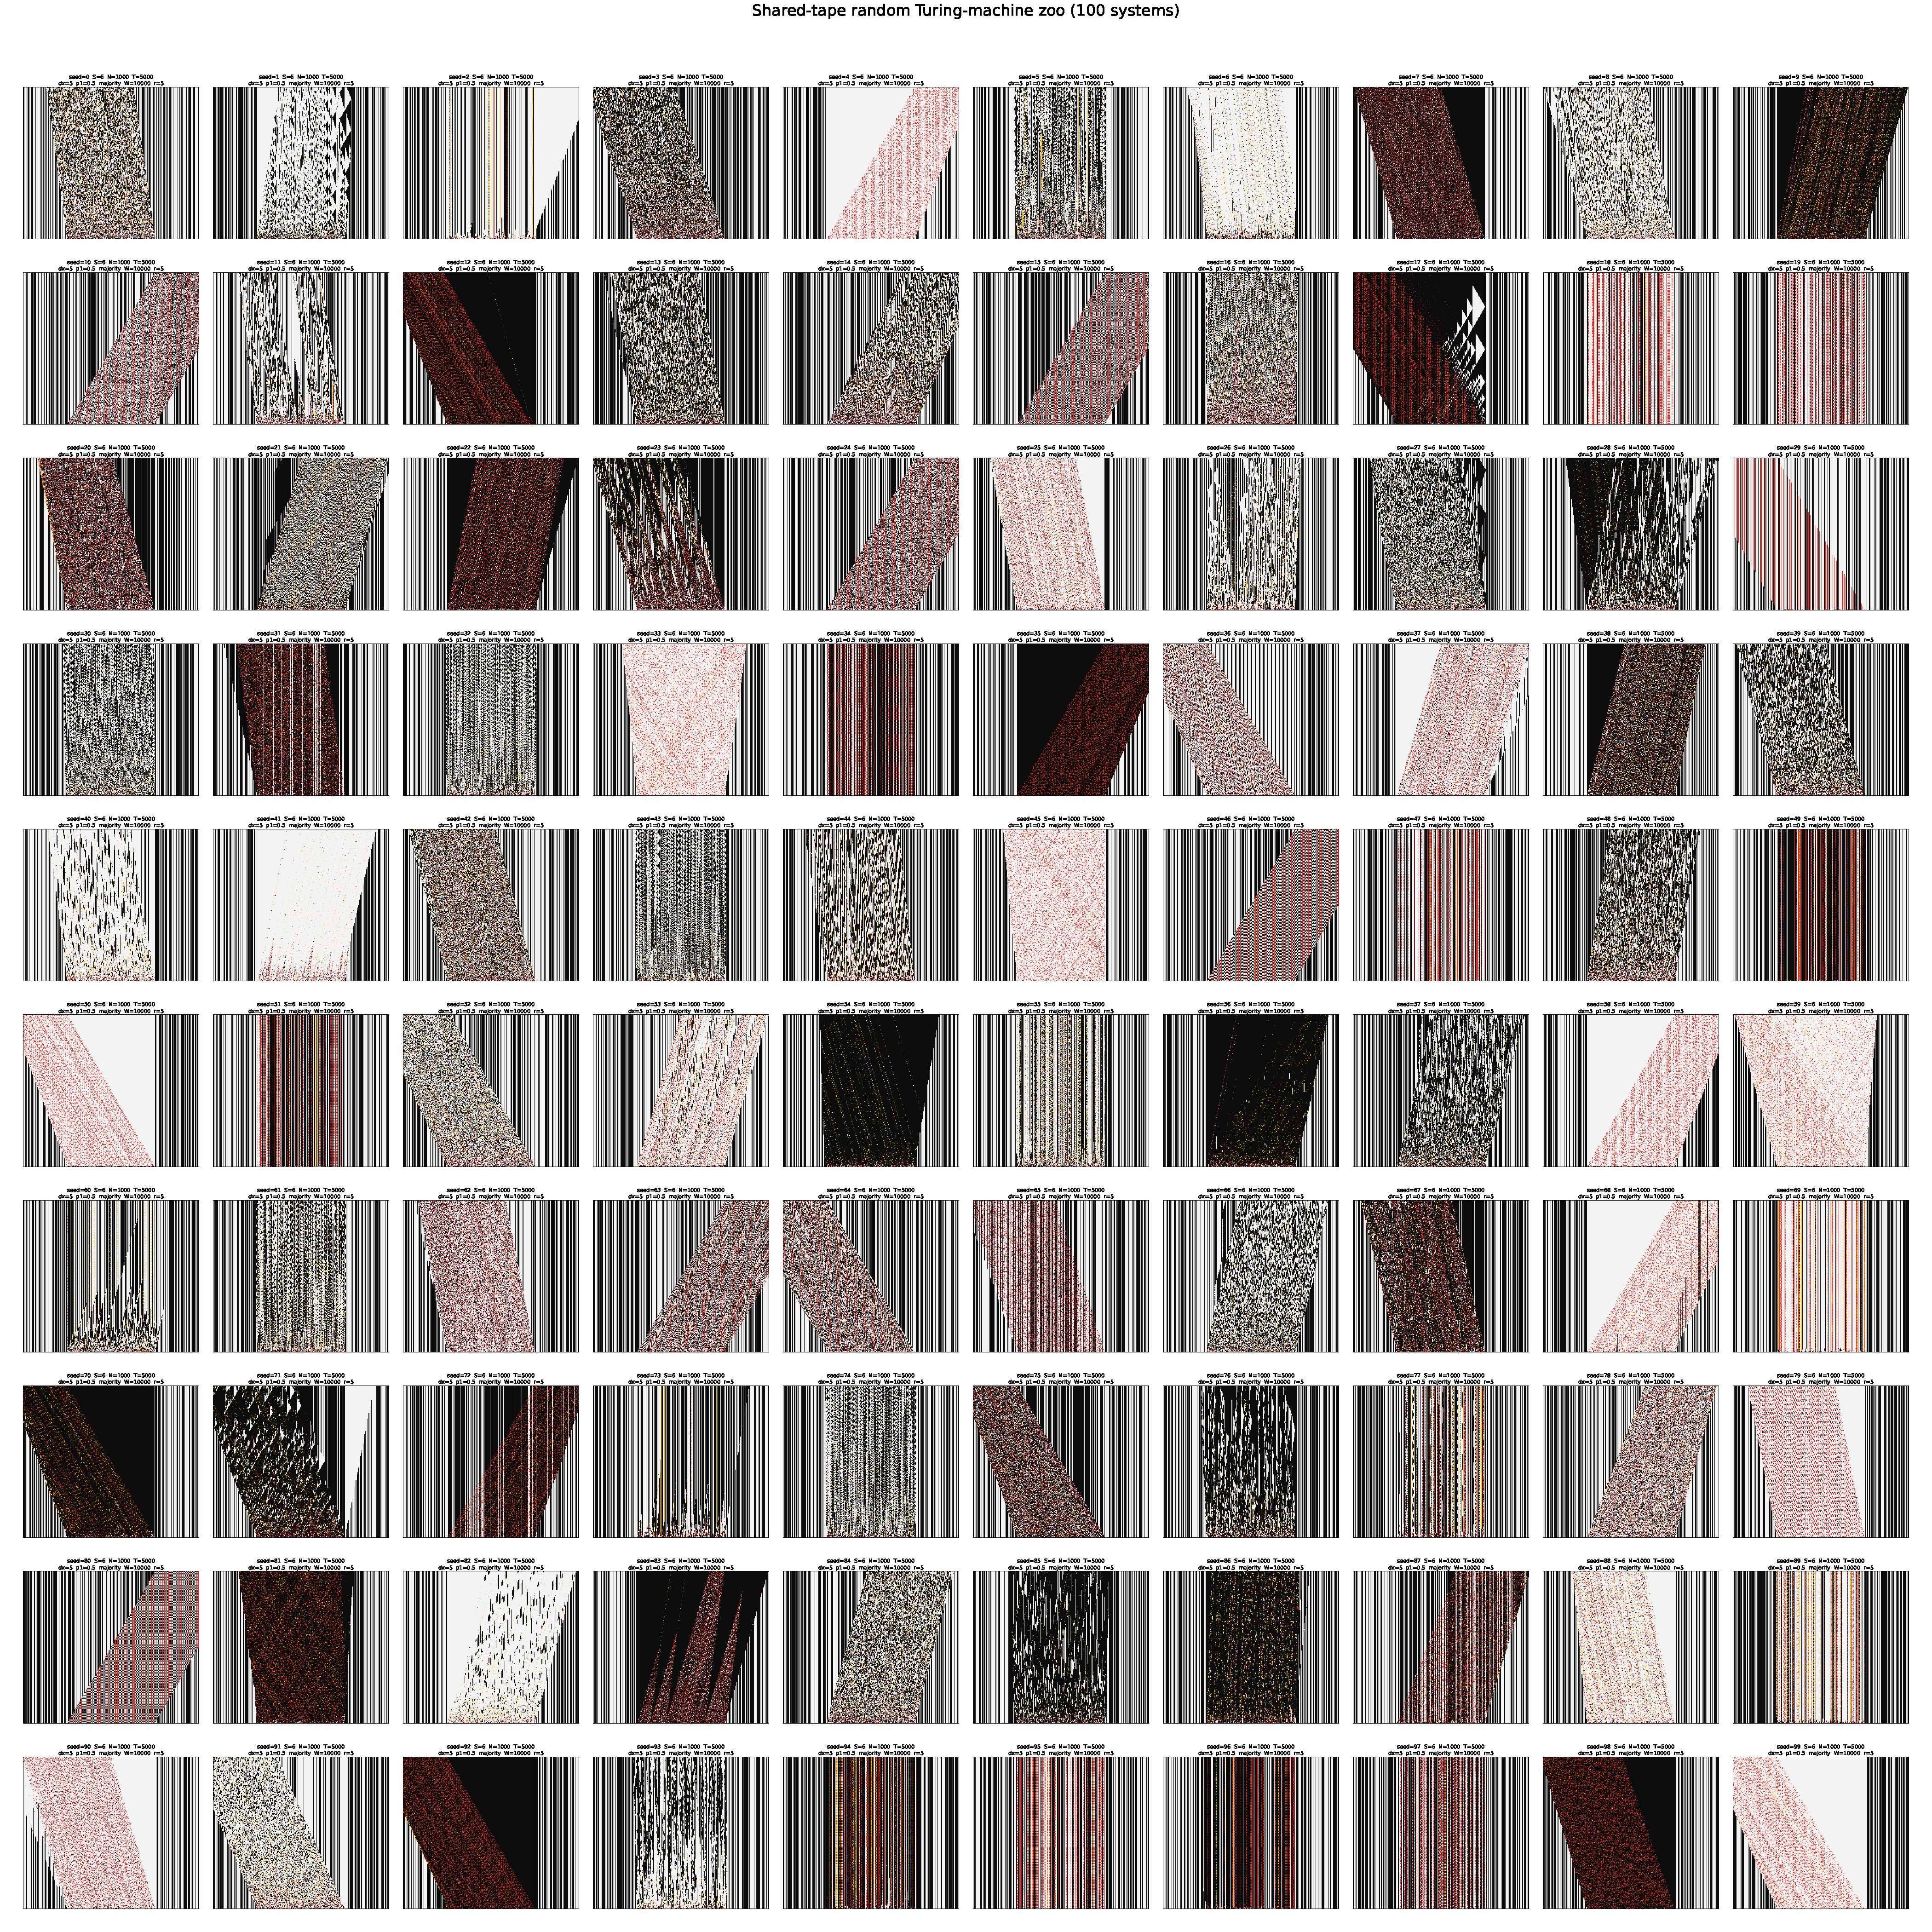
\includegraphics[width=\textwidth]{zoo_tm6_fixed_states.pdf}
\caption{Six-state reference ensemble.  Each of the 100 panels, seeds
$0$--$99$, uses $N=1000$ identical copies of a random ${\rm TM}_6(2)$,
all initialized at $q_0^{(i)}=1$.  The initial tape is
Bernoulli-$(1/2)$ and the head spacing is five.  Runs last $T=5000$
synchronous steps with majority-vote writes and unchanged symbols on
ties; the unbounded tape is shown over $-5000\leq x\leq4999$.
Snapshots were recorded every five steps.  Relative to the three-state
ensemble, the state-space size changes and new transition tables are
sampled.  This grid is also the fixed-state reference for
Fig.~\ref{fig:zoo-six-random}.  Time runs upward; dark/light indicates
tape symbols and red/yellow indicates head occupancy.}
\label{fig:zoo-six-fixed}
\end{figure}

\clearpage
\begin{figure}[p]
\centering
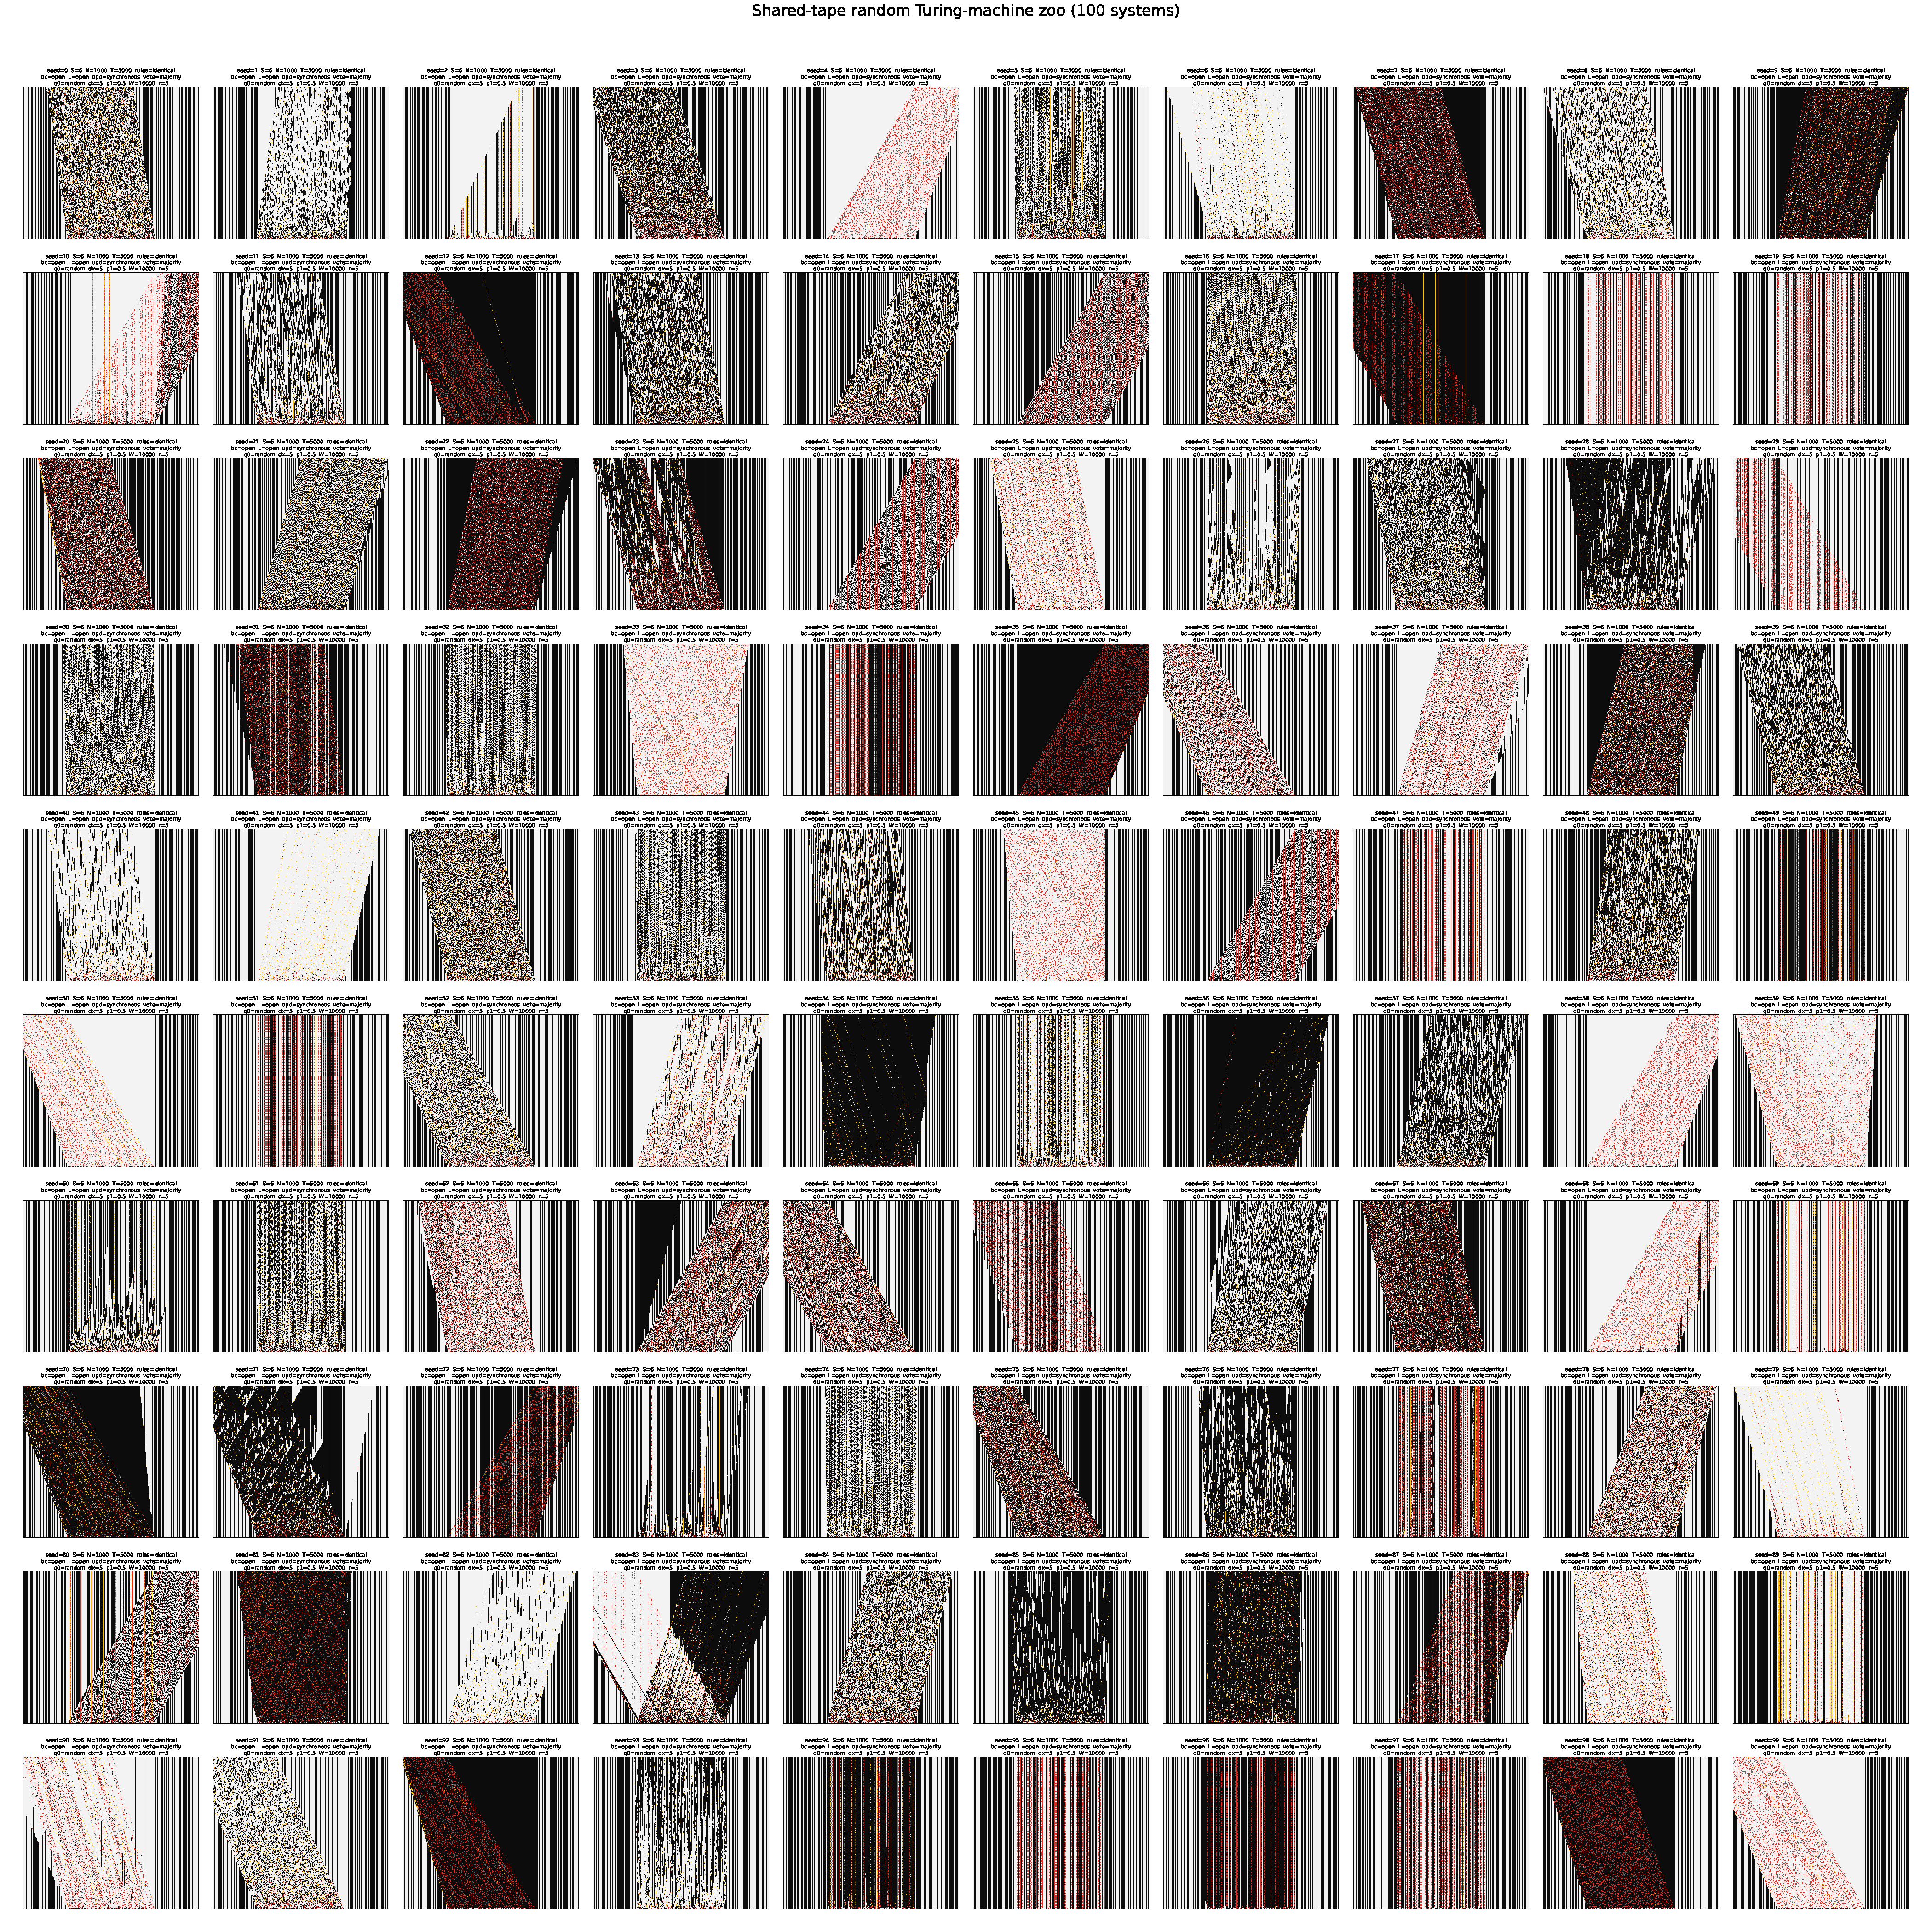
\includegraphics[width=\textwidth]{zoo_tm6_random_states.pdf}
\caption{Six-state machines with heterogeneous initial internal states.
The 100 panels, seeds $0$--$99$, share the same per-seed ${\rm TM}_6(2)$
tables as Fig.~\ref{fig:zoo-six-fixed}, but now
$q_0^{(i)}$ is independently uniform on $[6]$.  Each run contains
$N=1000$ identical-rule heads, a Bernoulli-$(1/2)$ tape, initial spacing
five, and $T=5000$ synchronous majority-vote steps (ties preserve the old
symbol).  The tape is unbounded; the plotted sites are
$-5000\leq x\leq4999$, recorded every five steps.
This separates diversity of initial head states from diversity of
transition tables.  Time runs upward; the red/yellow overlay indicates
single/multiple heads and does not encode their internal states.}
\label{fig:zoo-six-random}
\end{figure}

\clearpage
\begin{figure}[p]
\centering
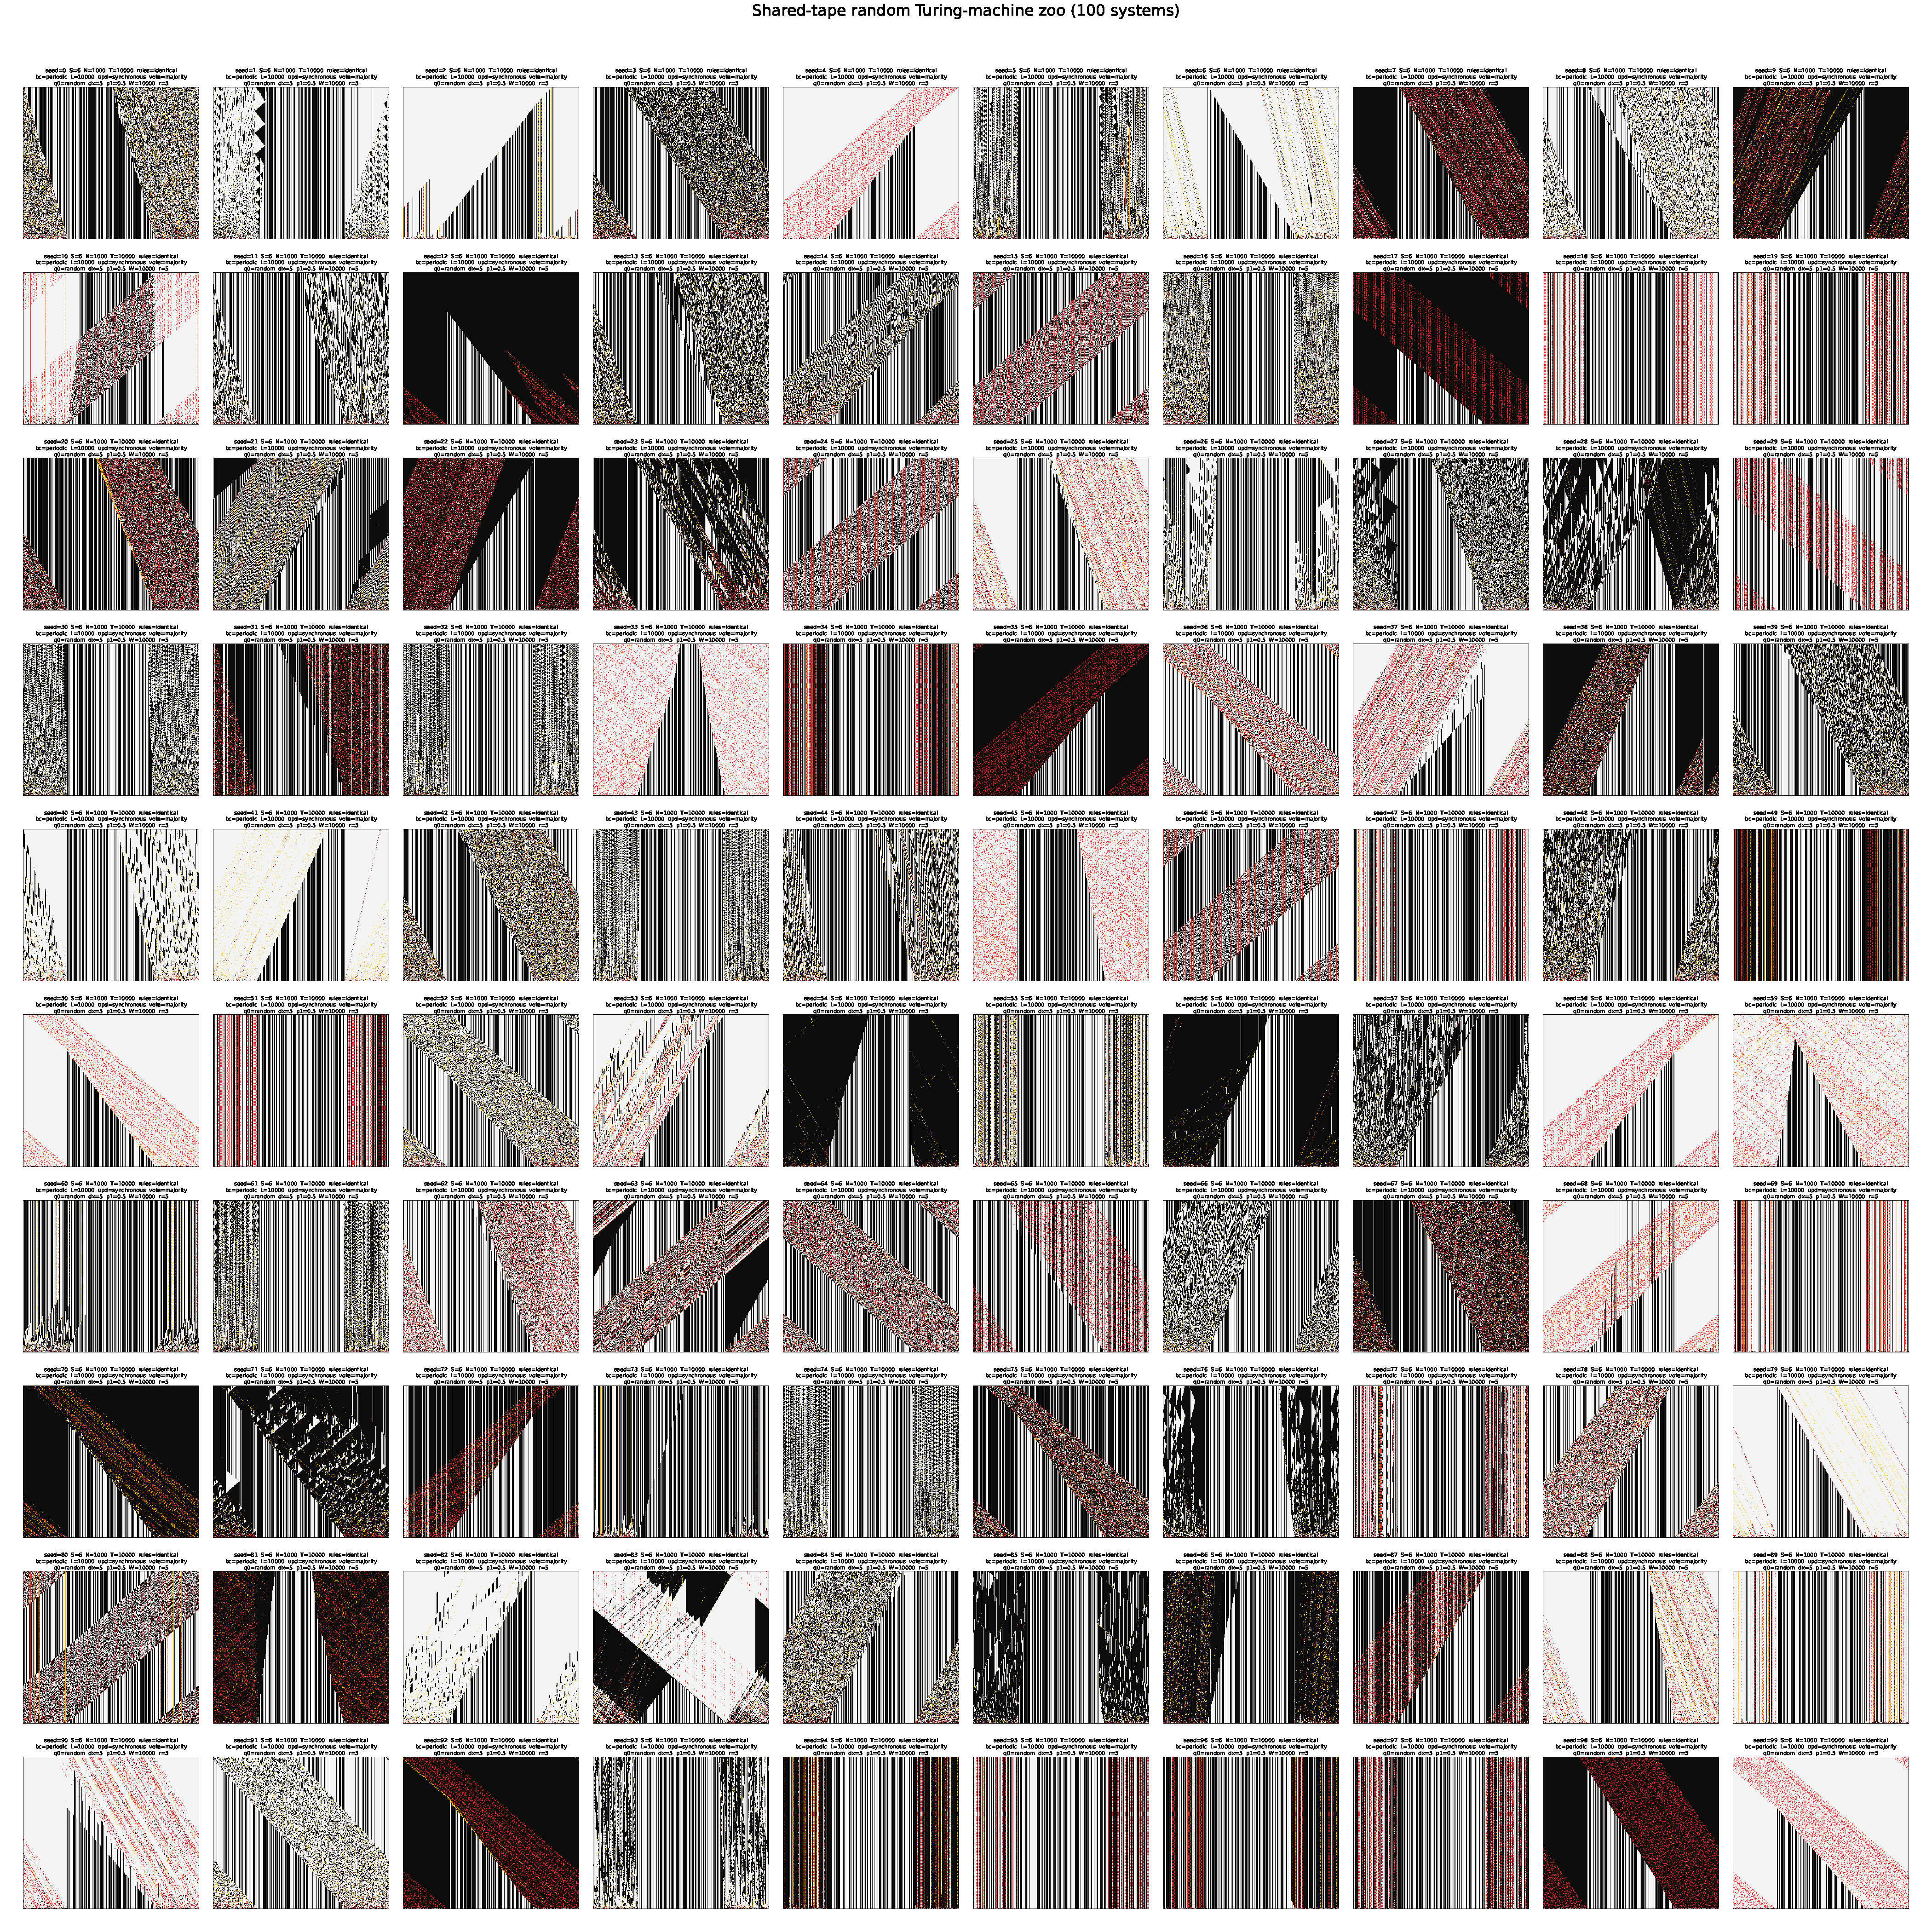
\includegraphics[width=\textwidth]{zoo_tm6_random_states_periodic.pdf}
\caption{Longer periodic runs of the six-state, random-initial-state
ensemble.  Seeds $0$--$99$ retain the transition tables of
Fig.~\ref{fig:zoo-six-random}, with $N=1000$ identical ${\rm TM}_6(2)$
heads, $q_0^{(i)}$ uniform on $[6]$, $p_1=1/2$, and initial spacing five.
Here the full ring $L=10000$ is shown for $T=10000$ synchronous steps,
using majority-vote writes with unchanged symbols on ties and recording
every five steps.  Both the geometry and duration differ from the
unbounded $T=5000$ runs; these are new periodic realizations, not
continuations of the earlier tapes.  Time runs upward.  Trajectories can
wrap across the spatial edges; those edges are not absorbing boundaries.}
\label{fig:zoo-six-periodic}
\end{figure}

\clearpage
\begin{figure}[p]
\centering
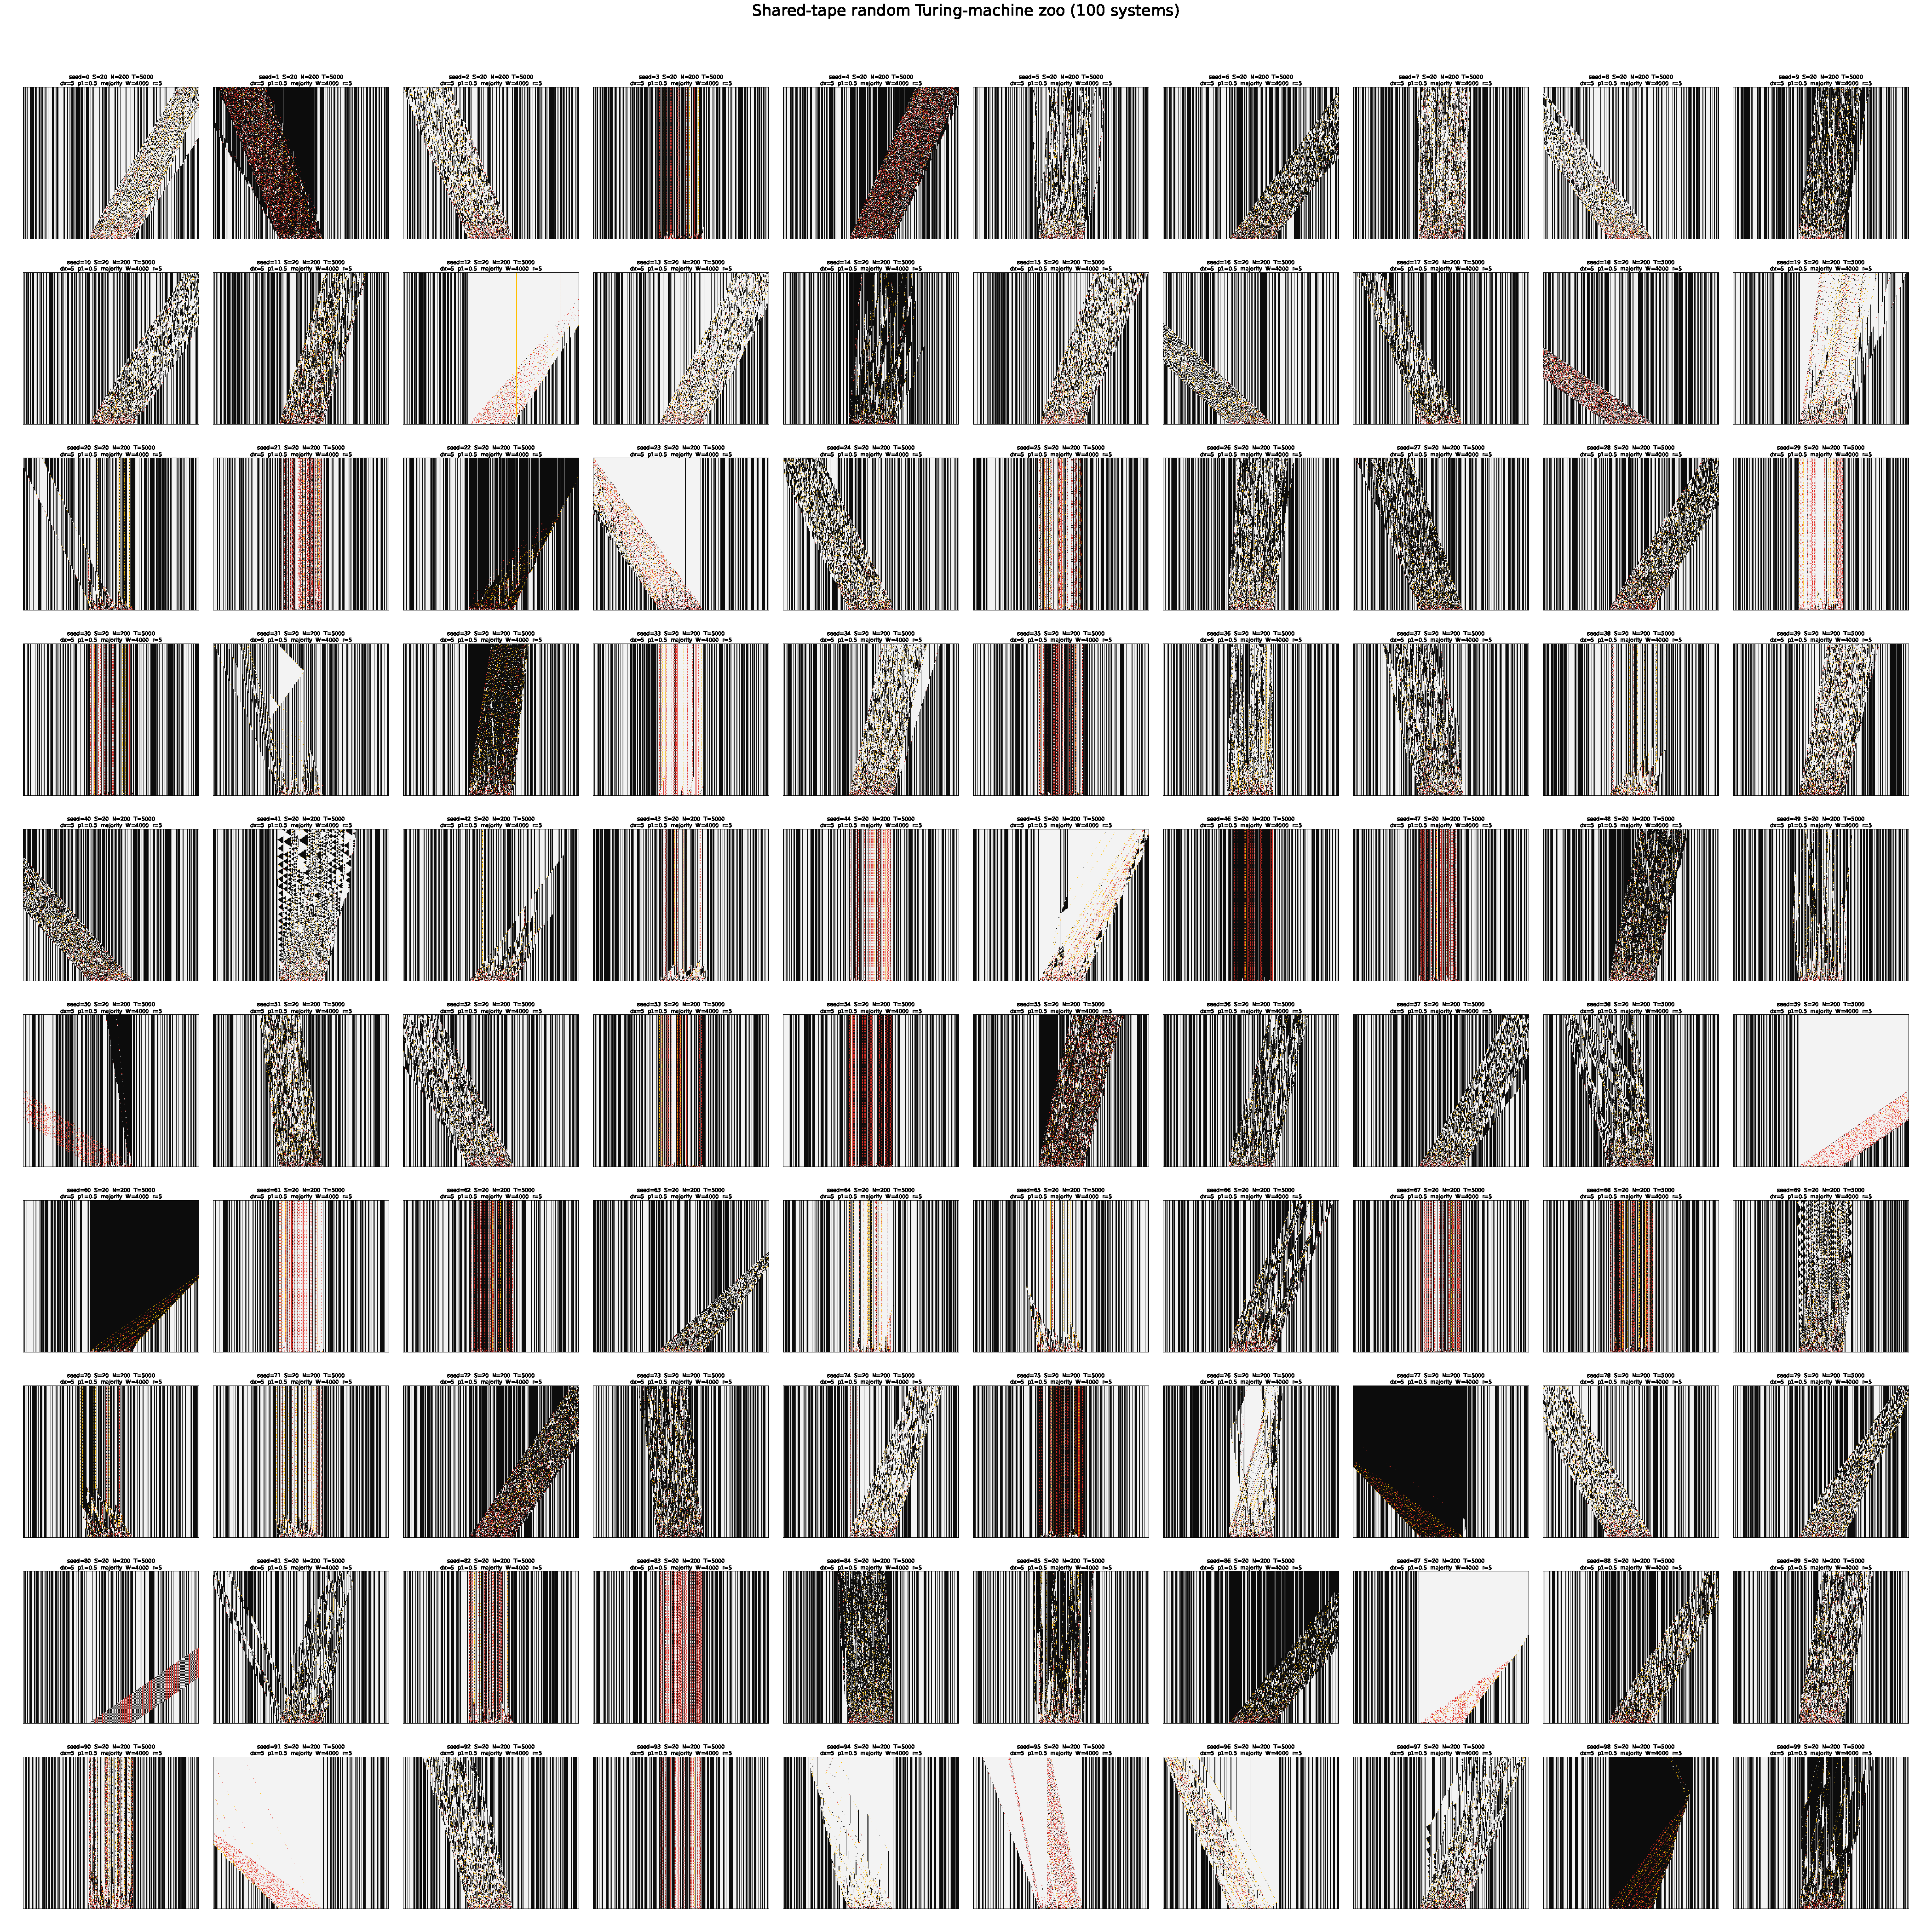
\includegraphics[width=\textwidth]{zoo_tm20_N200.pdf}
\caption{Original twenty-state zoo with $N=200$ heads.  Each of the 100
panels, seeds $0$--$99$, uses one random ${\rm TM}_{20}(2)$ shared by all
heads, with $q_0^{(i)}=1$, initial spacing five, and an independent-bit
tape with $p_1=1/2$.  Evolution lasts $T=5000$ synchronous steps with
majority-vote writes and unchanged symbols on ties.  The tape is
unbounded and the narrower display contains $-2000\leq x\leq1999$;
snapshots were recorded every five steps.  This is the smaller-population
reference for Fig.~\ref{fig:zoo-twenty-large}.  Time runs upward;
dark/light shows tape symbols and red/yellow shows single/multiple heads.
Heads crossing the display edge continue to evolve outside the image.}
\label{fig:zoo-twenty-small}
\end{figure}

\clearpage
\begin{figure}[p]
\centering
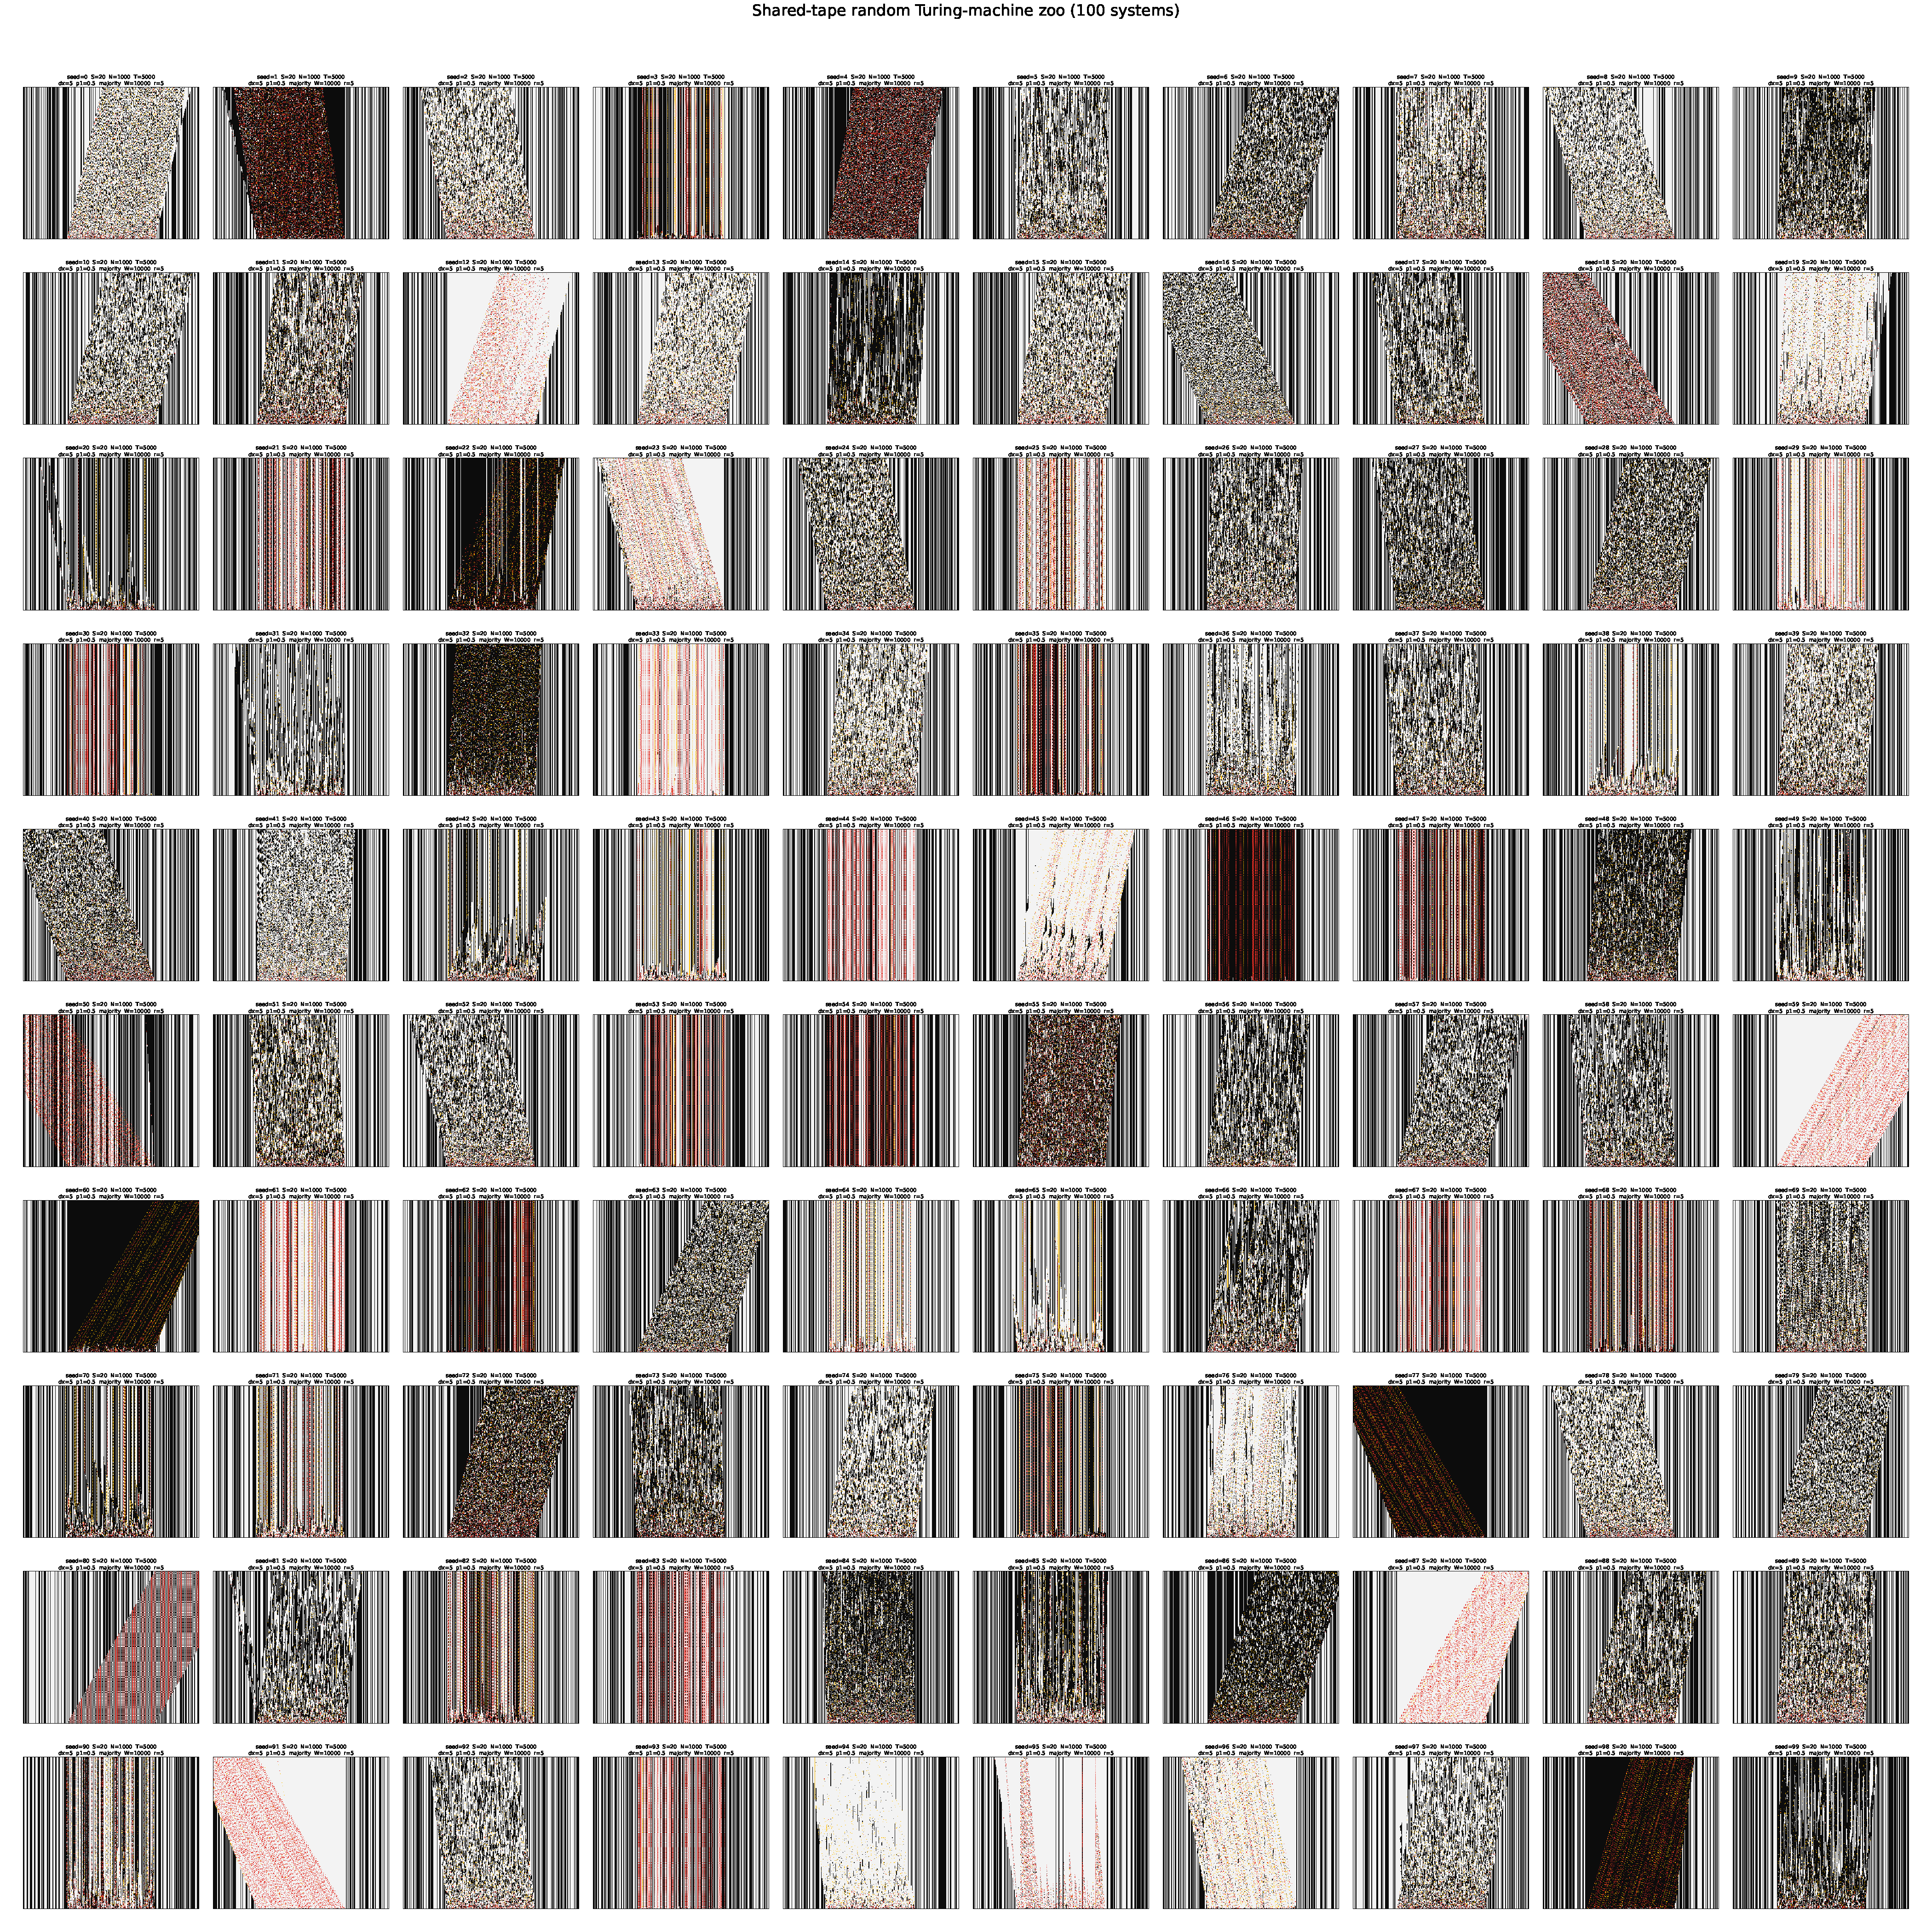
\includegraphics[width=\textwidth]{zoo_tm20_N1000.pdf}
\caption{Twenty-state zoo with the population increased to $N=1000$.
The 100 panels, seeds $0$--$99$, contain identical-rule
${\rm TM}_{20}(2)$ heads with $q_0^{(i)}=1$, initial spacing five, and
$p_1=1/2$.  The $T=5000$ updates are synchronous, using majority-vote
writes and unchanged symbols on ties.  The unbounded tape is now shown
over $-5000\leq x\leq4999$, with snapshots recorded every five steps.
Compared with Fig.~\ref{fig:zoo-twenty-small}, the initial occupied
interval and display window are larger while the local head spacing is
unchanged; this is not an increase of $N/L$ on a fixed periodic ring.
Time runs upward, with dark/light tape values and red/yellow occupancy.}
\label{fig:zoo-twenty-large}
\end{figure}

\clearpage
\begin{figure}[p]
\centering
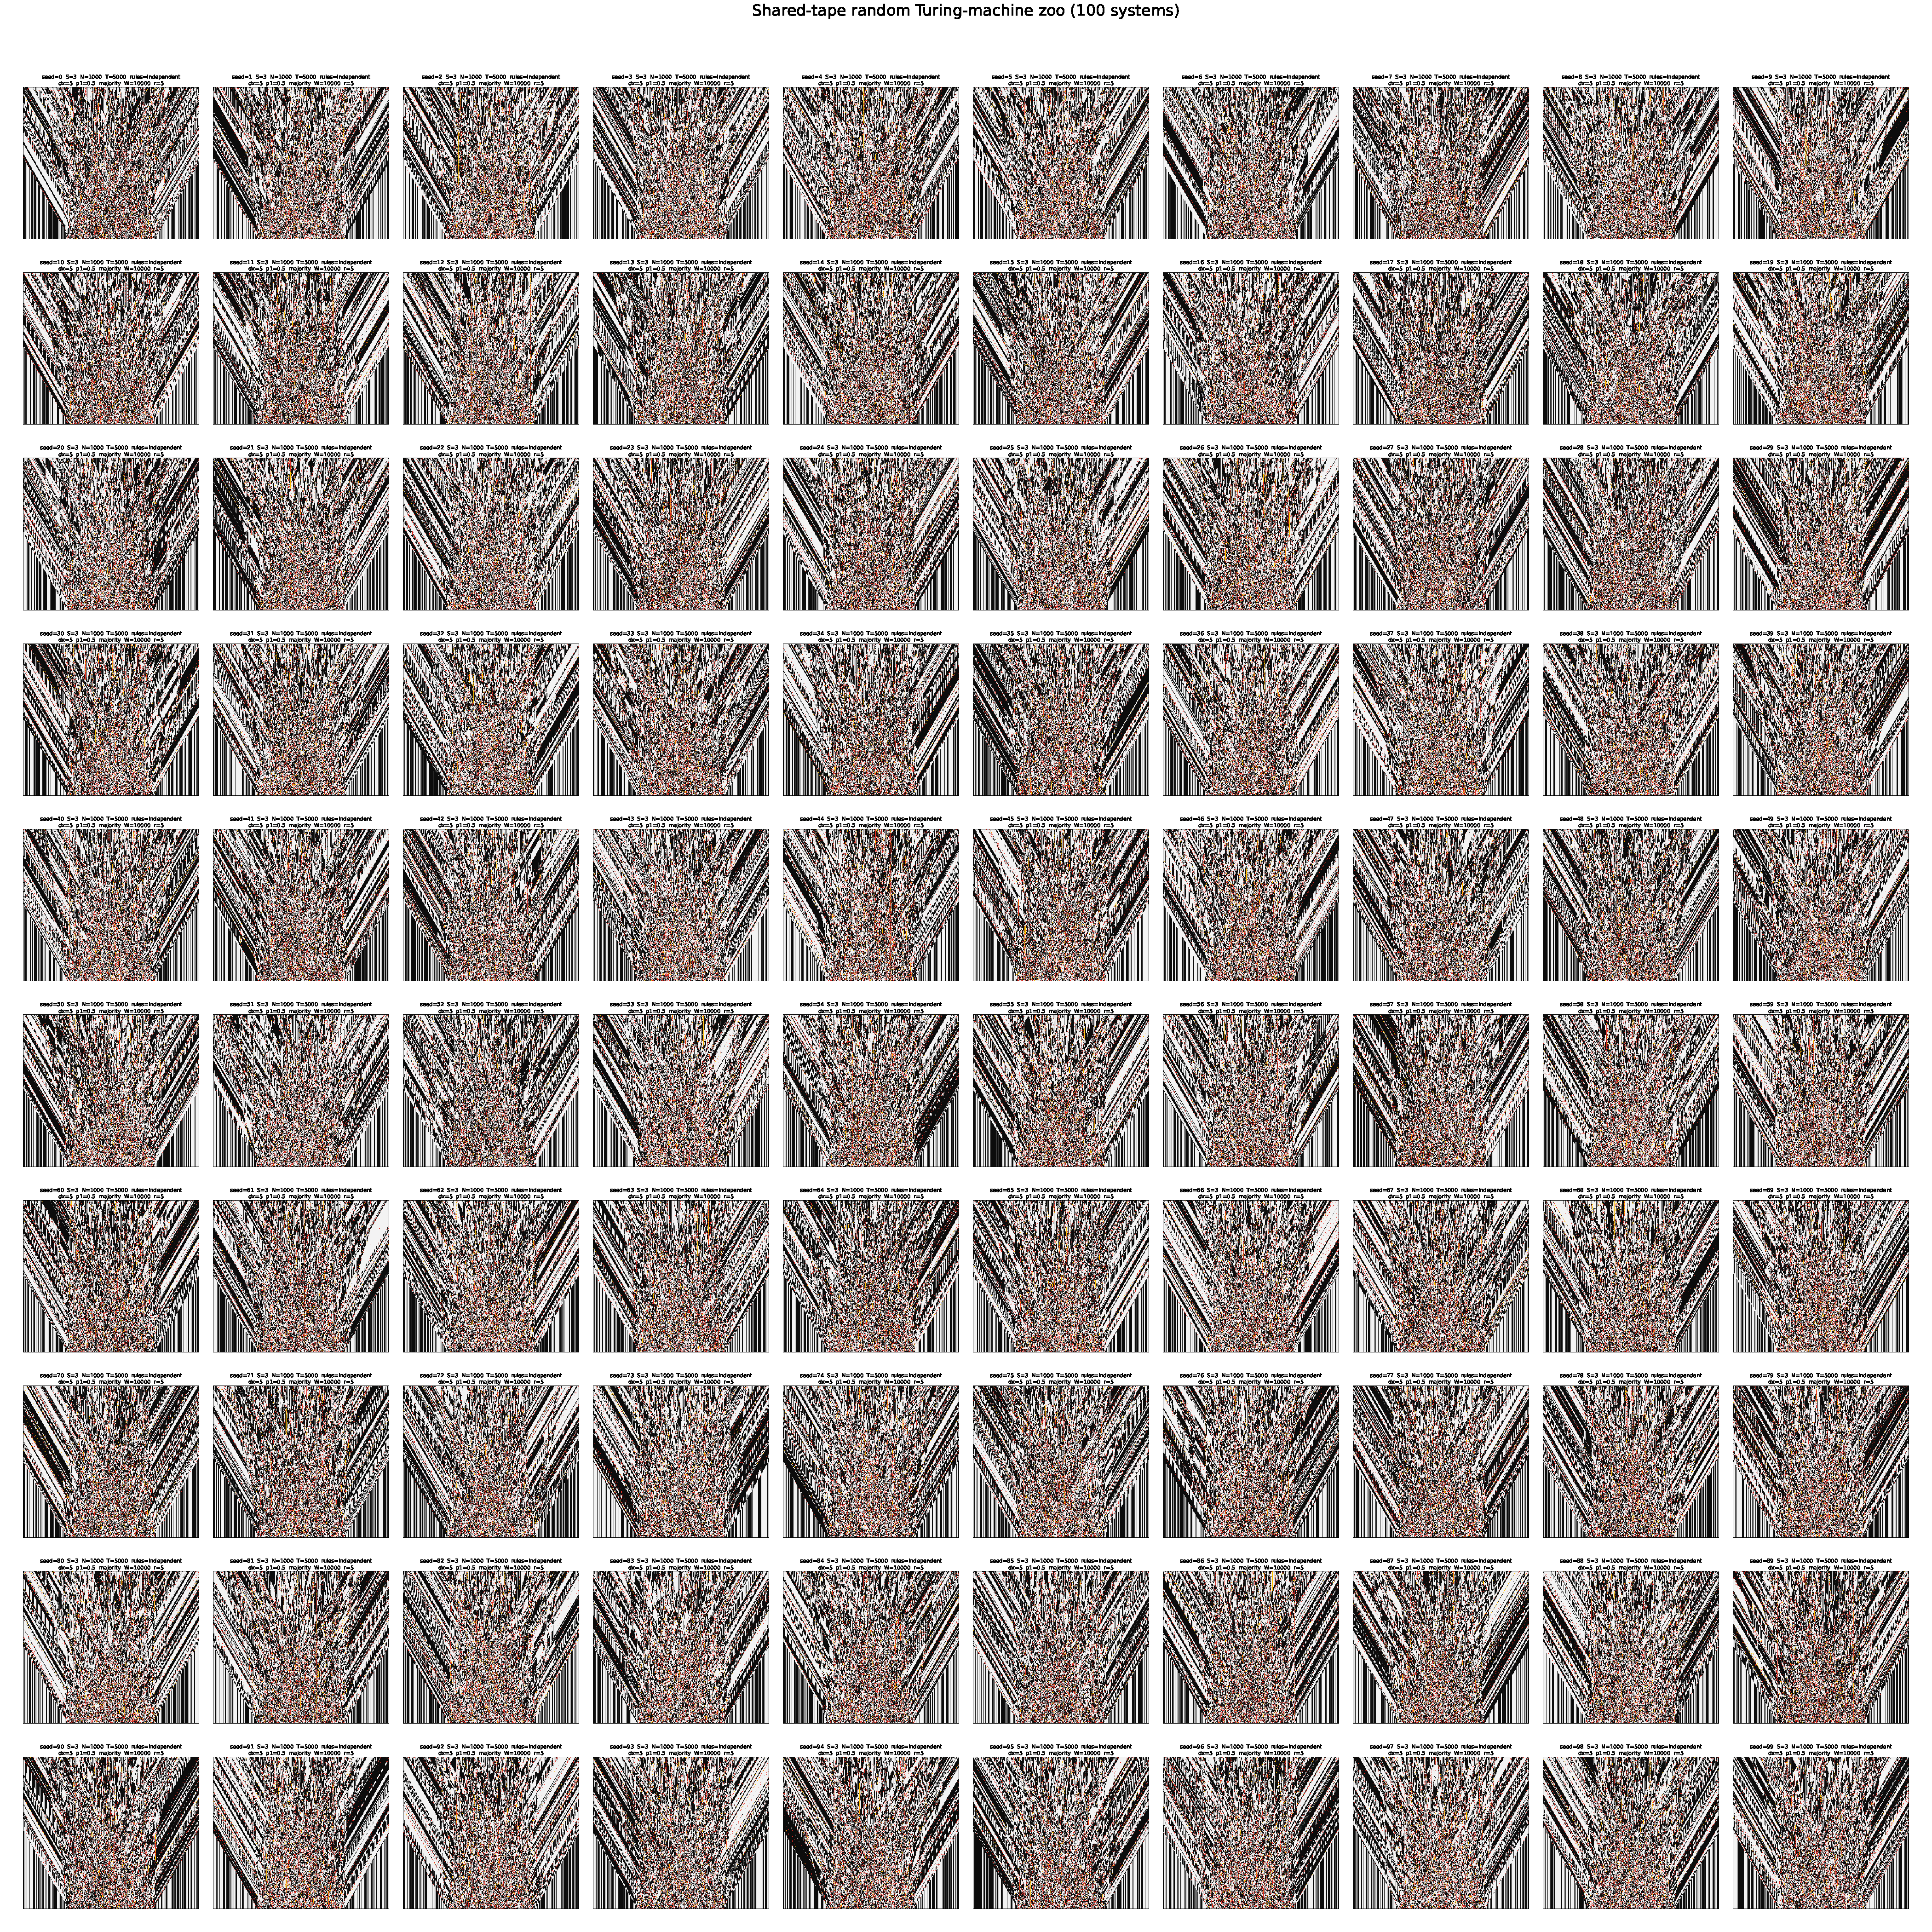
\includegraphics[width=\textwidth]{zoo_tm3_independent.pdf}
\caption{A heterogeneous gas of three-state machines on an unbounded
tape.  For each seed $0$--$99$, the $N=1000$ heads receive independently
sampled ${\rm TM}_3(2)$ transition tables $(M^{(i)},W^{(i)},S^{(i)})$;
all have $q_0^{(i)}=1$.  Initial spacing is five and $p_1=1/2$.
Each run lasts $T=5000$ synchronous steps with majority-vote writes and
unchanged symbols on ties.  The displayed window is
$-5000\leq x\leq4999$, with snapshots recorded every five steps.
Unlike Fig.~\ref{fig:zoo-three-state}, disorder now occurs between heads
within each realization as well as between panels.  The tables stay
fixed in time.  Time runs upward; the common red/yellow overlay marks
occupancy and does not distinguish the individual machine rules.}
\label{fig:zoo-independent-open}
\end{figure}

\clearpage
\begin{figure}[p]
\centering
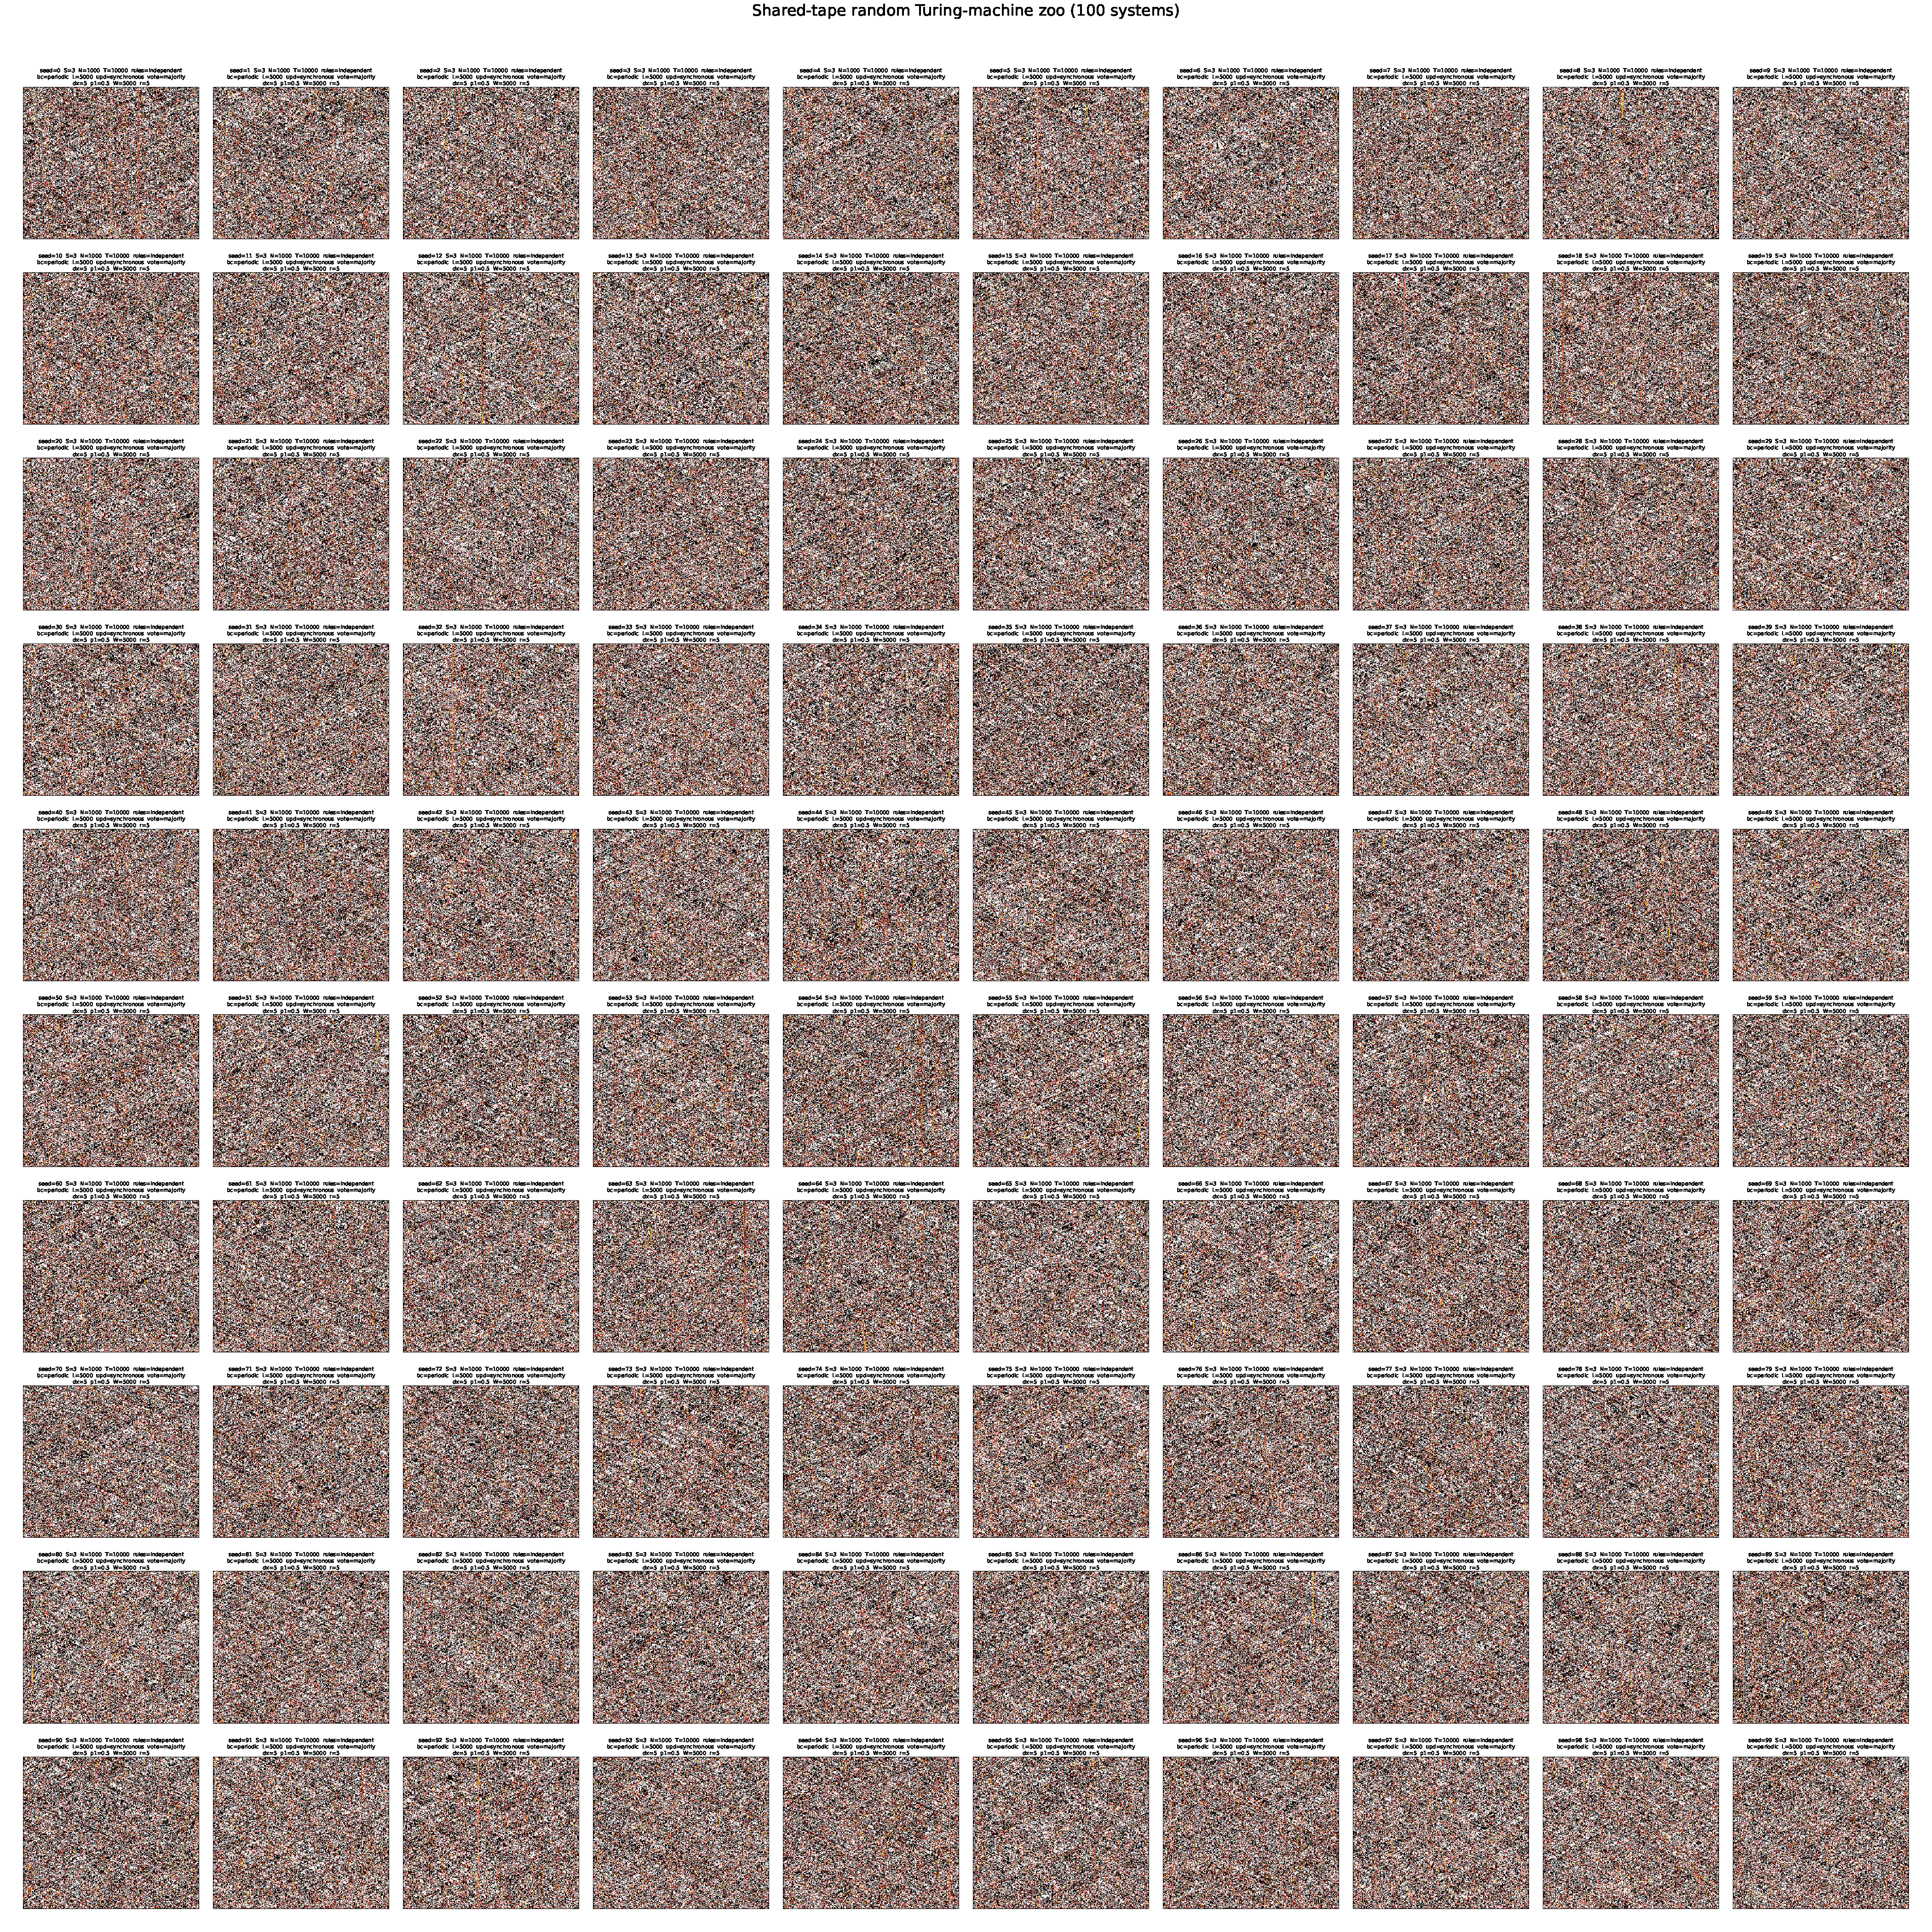
\includegraphics[width=\textwidth]{zoo_tm3_independent_periodic.pdf}
\caption{Heterogeneous three-state gas on a shorter periodic tape.
Each seed $0$--$99$ samples $N=1000$ independent ${\rm TM}_3(2)$ tables,
with $q_0^{(i)}=1$, $p_1=1/2$, and initial spacing five.  The full ring
has $L=5000$, hence $N/L=0.2$, and the duration is $T=10000$
synchronous steps.  Writes use majority vote with unchanged symbols on
ties; snapshots were recorded every five steps.  Relative to
Fig.~\ref{fig:zoo-independent-open}, the duration doubles and the
displayed spatial extent halves, while periodic wrapping replaces the
unbounded geometry.  The texture shown by these overviews alone does
not establish thermalization.  Time runs upward; dark/light represents
tape symbols and red/yellow represents single/multiple heads.}
\label{fig:zoo-independent-periodic}
\end{figure}

\clearpage
\begingroup
\raggedright
\bibliographystyle{unsrtnat}
\bibliography{tm-stat-mech}
\endgroup

\end{document}
